\documentclass{ieeeaccess}

% The ieeeaccess class selects fonts with \fontseries{n}, which is not a valid
% series. Map it to the regular series to avoid "Font shape undefined" warnings.
\begingroup
\fontencoding{T1}\fontfamily{ptm}\selectfont
\fontfamily{phv}\selectfont
\fontfamily{pcr}\selectfont
\endgroup
\DeclareFontShape{T1}{ptm}{n}{n}{<->ssub*ptm/m/n}{}
\DeclareFontShape{T1}{ptm}{n}{it}{<->ssub*ptm/m/it}{}
\DeclareFontShape{T1}{ptm}{n}{sl}{<->ssub*ptm/m/sl}{}
\DeclareFontShape{T1}{phv}{n}{n}{<->ssub*phv/m/n}{}
\DeclareFontShape{T1}{phv}{n}{sl}{<->ssub*phv/m/sl}{}
\DeclareFontShape{T1}{pcr}{n}{n}{<->ssub*pcr/m/n}{}
\let\proof\relax
\let\endproof\relax
\usepackage{amsmath,amssymb,amsthm,mathtools}
\usepackage{cite}
\usepackage{booktabs,array,tabularx}
\usepackage{graphicx}
\usepackage[ruled,vlined,linesnumbered]{algorithm2e}
\usepackage{enumitem}
\usepackage{textcomp}
\usepackage{microtype}
\usepackage{xurl}
\usepackage[hidelinks,bookmarks=false]{hyperref}
\usepackage[capitalize,nameinlink]{cleveref}

\theoremstyle{plain}
\newtheorem{theorem}{Theorem}
\newtheorem{proposition}[theorem]{Proposition}
\newtheorem{lemma}[theorem]{Lemma}
\newtheorem{corollary}[theorem]{Corollary}
\newtheorem{observation}[theorem]{Observation}
\theoremstyle{definition}
\newtheorem{definition}[theorem]{Definition}
\newtheorem{example}[theorem]{Example}
\newtheorem{remark}[theorem]{Remark}
\crefname{observation}{Observation}{Observations}
\Crefname{observation}{Observation}{Observations}

\newcommand{\F}{\mathbb{F}}
\newcommand{\Ftm}{\F_{2^m}}
\newcommand{\Red}{\operatorname{Red}}
\newcommand{\dX}{\operatorname{dXOR}}
\newcommand{\CX}{\operatorname{CX}}
\newcommand{\xor}{\oplus}
\SetKwInOut{Input}{Input}\SetKwInOut{Output}{Output}\SetKw{KwAnd}{and}
\SetAlFnt{\small}

\def\xfigwd{0pt}

\begin{document}
\bstctlcite{IEEEexample:BSTcontrol}
\history{Date of publication xxxx 00, 0000, date of current version xxxx 00, 0000.}
\doi{10.1109/ACCESS.2024.0429000}

\title{Efficient Closed-Form Reduction for Banegas' Second Family of Pentanomials}

\author{\uppercase{Marcos Tomaszewski}\authorrefmark{1},
\uppercase{Ricardo Custódio}\authorrefmark{1},
\uppercase{Gustavo Banegas}\authorrefmark{2},
and \uppercase{Daniel Panario}\authorrefmark{3},
\IEEEmembership{Senior~Member,~IEEE}}

\address[1]{Laboratório de Segurança em Computação (LabSEC), Departamento de Informática e
Estatística, Universidade Federal de Santa Catarina, Florianópolis, SC, Brazil}
\address[2]{GRACE Team, Inria Saclay, and LIX, École Polytechnique, Institut Polytechnique de Paris,
Palaiseau, France}
\address[3]{School of Mathematics and Statistics, Carleton University, Ottawa, ON, Canada}

\tfootnote{The work of M.~Tomaszewski was supported by a master's scholarship from
the Conselho Nacional de Desenvolvimento Científico e Tecnológico (CNPq), Brazil.
The work of D.~Panario was supported in part by the Natural Sciences and
Engineering Research Council of Canada (NSERC) under Grant RGPIN-2024-05342.}

\markboth
{Tomaszewski \headeretal: Efficient Closed-Form Reduction for Banegas' Second Family of Pentanomials}
{Tomaszewski \headeretal: Efficient Closed-Form Reduction for Banegas' Second Family of Pentanomials}

\corresp{Corresponding author: Marcos Tomaszewski (e-mail: marcos.tomaszewski@posgrad.ufsc.br).}

\begin{abstract}
In polynomial-basis arithmetic over \(\F_{2^m}\), the irreducible polynomial that defines the
field determines the cost of modular reduction and, with it, the cost of field
multiplication. Using a greedy XOR-counting heuristic, Banegas identified two families of
pentanomials with low reduction cost. The first family has since been analyzed, but the
second one,
\(f_{b,c}(x)=x^{b+2c}+x^{b+c}+x^b+x^c+1\) with \(b>c\ge1\), was left open because its
reduction has a less transparent structure. This paper closes that gap. For \(m=b+2c\), we
derive a closed form for the quotient of the polynomial division, written in terms of comb
sums of stride \(3c\), and turn it into an explicit reduction circuit with at most
\(3m-c-3\) XOR gates and depth at most \(\lfloor (m-2)/(3c)\rfloor+4\). This circuit is not
optimal. A second construction splits the reduction into \(c\) independent chains and
uses \(3m-3-N(b,c)\) XOR gates, where \(N(b,c)\approx(m-c)/3\); it is shorter whenever
\(b\ge4c+1\). Both constructions approach \(8m/3\) gates, at opposite ends of the
range of \(c\). Members built from five small base pentanomials split into independent
strips and admit even shorter programs, proved optimal with a SAT solver. We
verified both constructions symbolically for all 201,117 members with \(m\le1100\). An
irreducibility census for \(5\le m\le1100\) found irreducible members in 720 degrees, 288 of
which have no irreducible trinomial. Wherever both families have irreducible members, in 405
degrees, the second family is cheaper, by \(9.7\%\) on average. At the NIST degrees 163
and 571, the best members need 440 and 1,528 XOR gates, against 571 and 2,003 for the NIST pentanomials.
\end{abstract}

\begin{keywords}
Binary finite fields, bit-parallel multipliers, irreducible pentanomials, modular
reduction, polynomial basis, XOR circuit complexity.
\end{keywords}

\titlepgskip=-21pt

\maketitle

% ==================================================================
\section{Introduction}\label{sec:intro}
% ==================================================================
\PARstart{F}{inite} fields play an important role in cryptography and
error-correcting codes \cite{LidlNiederreiter1997,HMV2004}. Two types are
particularly relevant in practical implementations: prime fields $\F_p$, where
$p$ is a large prime, and binary extension fields $\Ftm\cong\F_2[x]/(f)$, where
$f$ is an irreducible polynomial of degree $m$. Arithmetic in prime fields
relies on multiprecision integer operations, often taking advantage of carefully
chosen primes to simplify modular reduction. In binary fields, addition requires
only bitwise XOR operations, while multiplication consists of a carry-less
polynomial product followed by reduction modulo $f$.

Several representations are available for binary fields, including polynomial,
normal, shifted and Montgomery bases, as well as towers of subfields. In a
polynomial basis, the multiplication of two polynomials does not depend on the
choice of $f$, but the subsequent reduction does. The selection of the
irreducible polynomial can therefore have a substantial impact on implementation
cost, particularly in terms of circuit area, delay and energy consumption. It
also affects the number of operations required in bitsliced software
implementations.

Although recent standardization efforts in elliptic curve cryptography have
favored prime fields, binary fields remain relevant in several cryptographic
constructions. NIST SP 800-186 retains prime-field curves, introduces Edwards
curves and deprecates the previously standardized binary-field curves
\cite{SP800186,FIPS1865}. Those binary curves used trinomials of degrees $233$
and $409$, and pentanomials of degrees $163$, $283$ and $571$. Outside elliptic
curve cryptography, binary fields continue to appear in widely used algorithms
and more recent proposals. AES uses $\F_{2^8}$ \cite{FIPS197}, while GCM
performs authentication using a degree-$128$ pentanomial
\cite{SP80038D,GueronKounavis2010}. Classic McEliece employs fields of degrees
$12$ and $13$ \cite{ClassicMcEliece2022,McBits2013}, and the post-quantum
signature scheme FAEST uses $\F_{2^\lambda}$ \cite{FAEST2023}. Towers of binary
fields also appear in succinct argument systems \cite{DiamondPosen2025}. Beyond
cryptography, Reed-Solomon and BCH codes provide further examples of
applications in which efficient binary-field arithmetic is important
\cite{Paar1997}.

The cost of polynomial reduction depends strongly on the number and positions of
the nonzero coefficients of $f$. Irreducible trinomials are especially
attractive, since reduction can be implemented using $2m-2$ XOR gates
\cite{SunarKoc1999,Wu2002}. However, irreducible trinomials do not exist for
every degree. In particular, Swan's theorem rules them out when $m\equiv0\pmod
8$, as well as for many odd degrees satisfying $m\equiv\pm3\pmod 8$
\cite{Swan1962}. Pentanomials are a natural alternative in these cases, and
considerable effort has been devoted to identifying families that permit
efficient reduction or multiplication
\cite{HasanWangBhargava1992,RodriguezKoc2003,
ReyhaniHasan2004,Cilardo2013,Imana2018,BCP2019}.

An earlier investigation of this problem was carried out by Banegas in his
master's thesis at LabSEC/UFSC \cite{Banegas2015}. Using a greedy XOR-counting
algorithm called \emph{Conta-XOR}, he examined all irreducible pentanomials of
degrees $19$ and $163$ and identified two families with particularly low
reduction costs:
\begin{align*}
&\text{(first)} &&
x^{2b+c}+x^{b+c}+x^b+x^c+1,\\
&\text{(second)} &&
x^{b+2c}+x^{b+c}+x^b+x^c+1.
\end{align*}
The first family was subsequently studied by Banegas, Custódio and Panario, who
established a reduction cost of $3m-2$ XOR gates, decreasing to
$\tfrac{12}{5}m-1$ when $b=2c$ \cite{BCP2019}. The second family, however, was
left without a corresponding analysis. Banegas observed that a better
understanding of its reduction process was needed and explicitly identified the
problem as a direction for future work \cite[Sec.~4.5]{Banegas2015}.

The present work addresses this open problem. We show that the second family
admits an algebraic structure that makes it possible to describe polynomial
reduction in closed form. The central observation is the identity
\[
(x^c+1)f=x^{b+3c}+x^b+x^{2c}+1,
\]
which provides a sparse multiple of the defining polynomial. Using this
identity, we derive an explicit expression for the quotient in polynomial
division and obtain a reduction algorithm whose XOR cost and circuit depth can
be bounded analytically.

The main contributions of this paper are:
\begin{enumerate}[leftmargin=*,itemsep=2pt]

\item We establish structural properties of the second
family of pentanomials, including the sparse-multiple identity used throughout
the analysis, and show that reduction splits into independent strips modulo a
base polynomial $G$ with $f_{b,c}(x)=G(x^{\gcd(b,c)})$. This explains why the
members built from five small base polynomials are cheaper, and we give
optimal strip programs for them (\cref{sec:family}).

\item We derive a closed-form expression for the quotient
$\lfloor D/f\rfloor$ using comb sums with stride $3c$ (\cref{thm:quotient}).

\item We construct an explicit reduction algorithm for
all $b>c\ge1$, requiring at most $3m-c-3$ XOR gates and having depth at most
$\lfloor(m-2)/(3c)\rfloor+4$. The corresponding multiplier requires $m^2+m-c-2$
XOR gates (\cref{thm:main,prop:depth,cor:mult}).

\item We show that this construction is not optimal and give a second one, based
on identities between sums of comb sums, which splits the reduction into $c$
independent chains. It uses exactly $3m-3-N(b,c)$ XOR gates, improves on
$3m-c-3$ whenever $b\ge4c+1$, and approaches $\tfrac83m$ when $c$ is small. For
several small members it matches the exact minima, or the best programs, found
with a SAT solver (\cref{thm:chain,tab:exact}).

\item We develop a word-level formulation with $O(\log(m/c))$ shift-and-XOR
operations and a gate-level variant of lower depth (\cref{sec:word}).

\item We compare the proposed reduction with the
greedy Conta-XOR algorithm. For generic members of the family, the closed-form
construction is never more expensive, accounts for the counts reported by
Banegas and improves them by exactly $2c-b$ XOR gates when $b<2c$
(\cref{sec:greedy}).

\item We perform an irreducibility census for degrees
up to $1100$, evaluate both constructions on it, characterize the irreducible
special members, and compare the resulting polynomials with those of the first
family, with type I and type II pentanomials, with irreducible trinomials and
with the NIST pentanomials (\cref{sec:comparison}).

\end{enumerate}

The remainder of the paper is organized as follows. \Cref{sec:background}
introduces the reduction cost model and reviews relevant previous results.
\Cref{sec:family} examines the second family and establishes its main algebraic
properties. The closed-form quotient is derived in \cref{sec:quotient} and used
to construct the reduction algorithm in \cref{sec:program}. \Cref{sec:chains}
presents the chain construction. \Cref{sec:word}
discusses word-level implementation and a lower-depth circuit variant.
Comparisons with Conta-XOR and other polynomial families are presented in
\cref{sec:greedy,sec:comparison}, followed by the discussion and conclusions in
\cref{sec:conclusion}.

% ==================================================================
\section{Background}\label{sec:background}
% ==================================================================

Let $f=x^m+g$, where $g(0)=1$ and $\deg g<m$. The product of two elements of
$\Ftm$ is a polynomial $D=\sum_{j=0}^{2m-2}d_jx^j$, which can be written as
\begin{equation}\label{eq:split}
\begin{gathered}
  D=L+x^mH,\qquad L=\sum_{i=0}^{m-1}d_ix^i,\\
  H=\sum_{s=0}^{m-2}h_sx^s,\qquad h_s=d_{m+s}.
\end{gathered}
\end{equation}
Reduction modulo $f$ produces $R=D\bmod f$. Since reduction is a fixed
$\F_2$-linear map, it can be represented by a matrix
$R_f\in\F_2^{m\times(2m-1)}$. Column $j$ of this matrix contains the
coefficients of $x^j\bmod f$. Thus, $R=R_f(d_0,\dots,d_{2m-2})^{\top}$, and each
output bit $r_i$ is obtained by XORing the inputs indicated by the corresponding
row of $R_f$.

The implementation cost of this linear map depends on how the XOR operations are
organized. A \emph{linear straight-line program} consists of instructions
$t\gets u\xor v$, where the operands are either input variables or previously
computed values. Its length is the number of XOR gates, while its \emph{depth}
is the maximum number of dependent gates along any computation path. Computing
each output independently requires $\dX(f)=\sum_i(w_i-1)$ XOR gates, where $w_i$
denotes the weight of row $i$ of $R_f$. We refer to this quantity as the
\emph{direct count}.

A smaller circuit may be obtained by sharing intermediate sums among different
outputs. For example, consider $y_0=x_1+x_2+x_3$, $y_1=x_1+x_2+x_4$, and
$y_2=x_2+x_3+x_4$. Computing the three sums independently requires six XOR
gates. By first computing $t=x_1\xor x_2$, the first two outputs become
$y_0=t\xor x_3$ and $y_1=t\xor x_4$. Together with the two gates required for
$y_2$, this gives a total of five gates.

We denote by $\Red(f)$ the minimum number of XOR gates required by a linear
straight-line program implementing $R_f$. Finding this minimum is NP-hard in
general \cite{BMP2013}, which motivates the use of heuristic methods. Paar's
greedy algorithm \cite{Paar1997} identifies the pair of operands occurring most
frequently among the output expressions, computes that pair once, and replaces
its occurrences with a temporary variable. Boyar and Peralta
\cite{BoyarPeralta2010} introduced a heuristic that also exploits cancellations
arising from the identity $v\xor v=0$. Further improvements have been proposed,
particularly for the linear layers of block ciphers
\cite{Kranz2017,Banik2019,TanPeyrin2020, Xiang2020,SunYangLi2025}. Exact
optimization using SAT solvers is possible for small instances
\cite{FuhsSK2010,Stoffelen2016}, but becomes impractical for the field degrees
considered in this work.

Conta-XOR, introduced independently by Banegas \cite[Ch.~4]{Banegas2015},
follows a greedy strategy similar to Paar's algorithm. It first constructs the
reduction matrix by repeatedly substituting $x^m$ with $g$ and canceling equal
terms in each output expression. The algorithm then selects the most frequent
pair of operands, replaces it with a temporary variable, and repeats this
procedure until no further sharing is possible. Its reported cost is the number
of temporary variables introduced plus the XOR operations remaining in the
output expressions. We denote this cost by $\CX(f)$.

For the present study, we implemented Conta-XOR independently and reproduced the
values reported by Banegas \cite{Banegas2015}. When several operand pairs have
the same frequency, our implementation uses lexicographic ordering to break
ties. This makes the results reproducible.

As a greedy method, Conta-XOR does not guarantee a minimum XOR count. A locally
favorable choice may prevent more efficient sharing in subsequent steps.
Moreover, its pair-substitution strategy does not exploit cancellations between
intermediate expressions. Despite these limitations, Conta-XOR was useful in
identifying pentanomials with low reduction costs, including the second family
studied here. Its output provides an upper bound on $\Red(f)$ rather than an
exact minimum. We compare these heuristic counts with those of our closed-form
construction in \cref{sec:greedy}.

Several families of irreducible polynomials admit reduction algorithms whose XOR
costs are known in closed form. \Cref{tab:known} summarizes the results relevant
to our comparison, including trinomials, equally spaced pentanomials, type I
pentanomials \cite{RodriguezKoc2003,ReyhaniHasan2004,Imana2018}, general
pentanomials with small middle exponents, and Banegas' first family. Type II
pentanomials $x^m+x^{n+2}+x^{n+1}+x^n+1$ \cite{RodriguezKoc2003} are compared in
\cref{sec:otherfamilies}.

\begin{table*}[t]
\centering\small
\caption{Reduction costs of families of irreducible
polynomials reported in the literature.}
\label{tab:known}
\begin{tabular}{@{}l l l l@{}}
\toprule
Polynomial & Condition & XORs for reduction & Ref.\\
\midrule
trinomial $x^m+x^a+1$
  & $a\le m/2$
  & $2m-2$
  & \cite{SunarKoc1999,Wu2002}\\
equally spaced
  $x^{4c}+x^{3c}+x^{2c}+x^c+1$
  & $m=4c$
  & $\tfrac74m-1$
  & \cite{HasanWangBhargava1992,Banegas2015}\\
type I pentanomial $x^m+x^{n+1}+x^n+x+1$
  & $2\le n\le m/2-1$
  & $3m-2$
  & \cite{ReyhaniHasan2004,BCP2019}\\
pentanomial $x^m+x^{k_3}+x^{k_2}+x^{k_1}+1$
  & $k_3\le m/2$
  & $4m-4$
  & \cite{ReyhaniHasan2004}\\
Banegas' first family
  $x^{2b+c}+x^{b+c}+x^b+x^c+1$
  & $b>c$
  & $3m-2$
  & \cite{BCP2019}\\
\quad the same, with $b=2c$
  & $m=5c$
  & $\tfrac{12}{5}m-1$
  & \cite{BCP2019}\\
\bottomrule
\end{tabular}
\end{table*}

For a schoolbook polynomial product, the partial products require $m^2$ AND
gates and $(m-1)^2$ XOR gates. The total XOR count of a multiplier is therefore
$(m-1)^2$ plus the cost of modular reduction. For Banegas' first family, this
gives $m^2+m-1$ XOR gates \cite{BCP2019}.


% ==================================================================
\section{The second family}\label{sec:family}
% ==================================================================

\begin{definition}\label{def:family}
Let $b>c\ge1$ be integers and set $m=b+2c$. The pentanomials
\[
  f_{b,c}(x)=x^{b+2c}+x^{b+c}+x^b+x^c+1
\]
form \emph{Banegas' second family}. Throughout the paper, $n=m-2$ denotes the
degree of the polynomial $H$ in \eqref{eq:split}.
\end{definition}

The restriction $b>c$, adopted in \cite{Banegas2015}, ensures that the five
exponents are distinct. In particular, $c<b<b+c<b+2c$.

\begin{proposition}\label{prop:basic}
Let $f=f_{b,c}$. Then:
\begin{enumerate}[label=(\roman*),itemsep=1pt]
  \item $x^m\equiv(x^b+1)(x^c+1)\pmod f$.

  \item $(x^c+1)f=x^{b+3c}+x^b+x^{2c}+1$.
  Consequently, $x^b(x^{3c}+1)\equiv(x^c+1)^2\pmod f$.

  \item $1\le c\le\lfloor(m-1)/3\rfloor$ and
  $b\equiv m\pmod 2$.

  \item If $\gamma=\gcd(b,c)>1$, then
  $f(x)=G(x^\gamma)$, where $G=f_{b/\gamma,\,c/\gamma}$ also belongs to the
  family. If $\gamma$ is even, then $f=G(x^{\gamma/2})^2$ and is therefore
  reducible.

  \item If $b=2c$, then $f$ is the equally spaced
  pentanomial $x^{4c}+x^{3c}+x^{2c}+x^c+1$.
\end{enumerate}
\end{proposition}

\begin{proof}
(i) Writing $f=x^m+g$, we have
\[
  g=x^{b+c}+x^b+x^c+1=(x^b+1)(x^c+1).
\]
Thus $x^m\equiv g\pmod f$.

(ii) Multiplication by $x^c+1$ gives
\[
  (x^c+1)f=x^{b+3c}+x^b+x^{2c}+1,
\]
since the remaining terms cancel in characteristic $2$. Reducing this identity
modulo $f$ yields
\[
  x^b(x^{3c}+1)\equiv x^{2c}+1
  =(x^c+1)^2\pmod f.
\]

(iii) Since $b\ge c+1$, we have $m=b+2c\ge3c+1$, which gives
$c\le\lfloor(m-1)/3\rfloor$. Also, $m-b=2c$, so $b$ and $m$ have the same
parity.

(iv) Let $b=\gamma b'$ and $c=\gamma c'$. Then $b'>c'\ge1$ and
\[
  f(x)=f_{b',c'}(x^\gamma)=G(x^\gamma).
\]
If $\gamma$ is even, the characteristic-$2$ identity
$G(x^{\gamma})=G(x^{\gamma/2})^2$ shows that $f$ is reducible.

(v) Substituting $b=2c$ into the definition gives the stated pentanomial.
\end{proof}

The identity in \cref{prop:basic}(ii) is central to the reduction method
developed in this paper. To obtain it, write
\[
  f=x^b(x^{2c}+x^c+1)+(x^c+1).
\]
Since
\[
  (x^c+1)(x^{2c}+x^c+1)=x^{3c}+1
\]
over $\F_2$, multiplication by $x^c+1$ produces a multiple of $f$ containing
only four nonzero terms. The resulting congruence can be expressed as
\[
  x^{s+b+3c}\equiv
  x^{s+b}+x^{s+2c}+x^s\pmod f,
  \qquad s\ge0.
\]
This relation allows a high-degree term to be replaced by three lower-degree
terms, with a reduction step of $3c$ in the leading exponent.

For example, taking $b=11$ and $c=2$ gives
\[
  f=x^{15}+x^{13}+x^{11}+x^2+1
\]
and
\[
  (x^2+1)f=x^{17}+x^{11}+x^4+1.
\]
Therefore,
\[
  x^{17}\equiv x^{11}+x^4+1\pmod f.
\]

A similar identity holds for Banegas' first family:
\[
  (x^b+1)f=x^{3b+c}+x^{2b}+x^c+1.
\]
The difference lies in the spacing between the leading exponents. For the first
family, the corresponding stride is $3b$, which exceeds the field degree
$m=2b+c$. For the second family, the stride is $3c<m$. Consequently, reduction
in the second family may involve several successive applications of the same
relation, particularly when $b$ is large relative to $c$.

This distinction becomes explicit in the closed-form quotient derived in
\cref{sec:quotient}. In the first family, the corresponding comb sums contain at
most one coefficient, whereas in the second family they may contain several. The
parameter $c$ therefore influences both the reduction cost and the depth of the
resulting circuit.

\begin{definition}[Special and generic members]
\label{def:special}
Let $\gamma=\gcd(b,c)$, and write $b=\gamma b'$ and $c=\gamma c'$. Then
$f_{b,c}(x)=G(x^\gamma)$, where the \emph{base polynomial} $G=f_{b',c'}$ has
degree $\kappa=b'+2c'$ (\cref{prop:basic}(iv)). A member of the family is called
\emph{special} if its base polynomial is one of
\[
  f_{2,1},\quad f_{3,1},\quad f_{4,1},\quad f_{5,1},\quad f_{3,2},
\]
that is, if $b/c\in\{\tfrac32,2,3,4,5\}$, or equivalently if $\deg G\le7$. All
other members are called \emph{generic}.
\end{definition}

The classification depends only on the ratio $b/c$, and not on the degree $m$.
Each of the five base polynomials produces special members $G(x^\gamma)$ in
every degree $m=\gamma\kappa$. For special members, $c'\le2$ and therefore
$\gamma\ge c/2$. The equally spaced case $b=2c$ corresponds to the base
polynomial $f_{2,1}=x^4+x^3+x^2+x+1$.

The reason for singling out these five base polynomials is structural. When
$\gamma>1$, reduction modulo $f$ splits into independent reductions modulo $G$,
and \cref{alg:main} respects this splitting.

\begin{proposition}[Strip decomposition]\label{rem:strips}
Let $f=f_{b,c}=G(x^\gamma)$ with $\gamma=\gcd(b,c)$, $G=f_{b',c'}$ and
$\kappa=\deg G$, so that $m=\gamma\kappa$. For $0\le\rho<\gamma$, call the set of indices
congruent to $\rho$ modulo $\gamma$ the \emph{strip} $\rho$.
\begin{enumerate}[label=(\roman*),itemsep=1pt]
  \item Reduction modulo $f$ splits into $\gamma$ independent reductions modulo
        $G$, one per strip. Strips $0,\dots,\gamma-2$ each reduce a polynomial
        of degree at most $2\kappa-1$, and strip $\gamma-1$ reduces a polynomial of
        degree at most $2\kappa-2$. Consequently,
        \[
          \Red(f)\le(\gamma-1)\,R_1(G)+R_2(G),
        \]
        where $R_1(G)$ and $R_2(G)$ are the lengths of any programs for these
        two reductions modulo $G$.
  \item Every gate of \cref{alg:main} combines operands from a single strip. On
        strip $\gamma-1$, after the relabeling $i\mapsto(i-\gamma+1)/\gamma$,
        it coincides with \cref{alg:main} for $G$ and uses $3\kappa-c'-3$ gates. On
        each of the other strips it uses $3\kappa-c'$ gates.
\end{enumerate}
\end{proposition}

\begin{proof}
(i) Write $D=\sum_{\rho=0}^{\gamma-1}x^\rho D_\rho(x^\gamma)$. Since $f$ involves only
powers of $x^\gamma$,
\[
  D\bmod f=\sum_{\rho=0}^{\gamma-1}x^\rho\bigl(D_\rho\bmod G\bigr)(x^\gamma),
\]
because every term on the right has degree less than $m$. The polynomial $D$ has
degree at most $2m-2=2\gamma\kappa-2$. Counting the indices $j\le2\gamma\kappa-2$ with
$j\equiv \rho\pmod\gamma$ shows that $D_\rho$ has degree at most $2\kappa-1$ for
$\rho\le\gamma-2$ and at most $2\kappa-2$ for $\rho=\gamma-1$.

(ii) All index shifts used in \cref{alg:main} are $c$, $b$, $b+c$ and $3c$,
which are multiples of $\gamma$, and the high coefficient $h_s$ is the input
$d_{m+s}$ with $m\equiv0\pmod\gamma$. Hence every gate stays within one strip.
On strip $\gamma-1$, write each index as $\gamma-1+\gamma i'$. A direct check
shows that every range condition of \cref{alg:main} for $(b,c)$ becomes the
corresponding condition for $(b',c')$; for example, $t+3c\le n$ becomes
$t'+3c'\le \kappa-2$, and the condition $u\le c-2$ on the index $u$ of $U_u$ becomes
$u'\le c'-2$. The program on this strip
is therefore \cref{alg:main} for $G$, with $3\kappa-c'-3$ gates. The same check,
with indices $\rho+\gamma i'$, shows that strips $0,\dots,\gamma-2$ run identical
programs up to relabeling. Since \cref{alg:main} has exactly
$3m-c-3=\gamma(3\kappa-c')-3$ gates (proof of \cref{thm:main}), each of these strips
uses $3\kappa-c'$ gates.
\end{proof}

\Cref{rem:strips}(ii) says that the closed form for $f$ is the closed form for
$G$ applied once per strip. Any saving over $3m-c-3$ must therefore come from a
strip, that is, from a reduction modulo $G$ that is shorter than the closed
form. Writing
\begin{align*}
  \delta_1(G)&=(3\kappa-c')-R_1(G),\\
  \delta_2(G)&=(3\kappa-c'-3)-R_2(G),
\end{align*}
\cref{rem:strips}(i) gives
\begin{equation}\label{eq:specialbound}
  \Red(f)\le 3m-c-3-(\gamma-1)\,\delta_1(G)-\delta_2(G).
\end{equation}
The saving grows linearly with $\gamma$, and hence with $m$, along each ratio
$b/c$.

\Cref{tab:base} lists the shortest strip programs for the five base
polynomials. They were found by greedy pair substitution with lexicographic and
randomized tie-breaking and, for $f_{4,1}$ and $f_{5,1}$, by an exact search with
a SAT solver (\cref{sec:greedy}). The SAT solver also proves that all values in
the table are optimal. Each program was composed over the strips and checked
symbolically against the reduction matrix of $f$ for all $\gamma$ with
$m\le1100$. For $f_{2,1}$ the bound is $7\gamma-1=\tfrac74m-1$, the known cost
of the equally spaced pentanomial (\cref{tab:known}); for $f_{3,1}$ it is
$12\gamma-2=\tfrac{12}5m-2$, and for $f_{4,1}$ it is $15\gamma-1=\tfrac52m-1$.

\begin{table}[t]
\centering\small
\caption{Optimal strip programs for the five base polynomials of
\cref{def:special}, compared with the closed form, and the resulting bound
\eqref{eq:specialbound} for $f=G(x^\gamma)$. Optimality of every value of
$R_1(G)$ and $R_2(G)$ was proved with a SAT solver.}
\label{tab:base}
\setlength{\tabcolsep}{4pt}
\begin{tabular}{@{}c c c c c c l@{}}
\toprule
$G$ & $\kappa$ & $R_2(G)$ & $3\kappa-c'-3$ & $R_1(G)$ & $3\kappa-c'$ & bound for $f$\\
\midrule
$f_{2,1}$ & $4$ & $6$  & $8$  & $7$  & $11$ & $\tfrac74m-1$\\
$f_{3,1}$ & $5$ & $10$ & $11$ & $12$ & $14$ & $\tfrac{12}5m-2$\\
$f_{4,1}$ & $6$ & $14$ & $14$ & $15$ & $17$ & $\tfrac52m-1$\\
$f_{5,1}$ & $7$ & $16$ & $17$ & $18$ & $20$ & $\tfrac{18}7m-2$\\
$f_{3,2}$ & $7$ & $16$ & $16$ & $18$ & $19$ & $\tfrac{18}7m-2$\\
\bottomrule
\end{tabular}
\end{table}

We applied the greedy search, with $200$ randomized runs per reduction, to all
$163$ reduced pairs $(b',c')$ with $4\le\kappa\le40$. Only the five base polynomials
of \cref{def:special} admit a strip program shorter than the closed form that
these heuristics can find. For every other pair, including the degree-$8$ pair
$(6,1)$, the best heuristic program matches or exceeds the closed form. This is
the reason for the threshold $\deg G\le7$. When $G$ is very small, the strip
reduction involves only a few outputs and at most seven quotient coefficients,
and there is room for groupings of the same sums that are shorter than the
uniform structure of \cref{alg:main}. In the extreme case $G=f_{2,1}$, which
divides $x^5+1$, reduction modulo $G$ is little more than a cyclic shift, and
\cref{alg:main} even computes some values twice; for the other four base
polynomials, all the values computed by \cref{alg:main} are distinct, and the
savings come from different groupings.

The classification should be read as a statement about what pair-substitution
heuristics find, not about $\Red(G)$. Generic members can also beat the closed
form. The chain construction of \cref{sec:chains} does so for every member with
$b\ge4c+1$, and an exact search gives $\Red(f_{6,1})=19$ and $\Red(f_{5,2})=21$,
one gate below the closed form (\cref{sec:greedy}). What sets the five base
polynomials apart is that their savings are found by simple heuristics and that
we have provably optimal strip programs for them.


% ==================================================================
\section{A closed form for the quotient}\label{sec:quotient}
% ==================================================================


Polynomial division can be expressed in terms of the coefficients of the
dividend, quotient and remainder.

\begin{lemma}[Division identities]\label{lem:division}
Let $f=x^m+\sum_{e\in S}x^e+1$, with $S\subseteq\{1,\dots,m-1\}$, and let
$Q=\lfloor D/f\rfloor=\sum_{j=0}^{n}q_jx^j$. Then
\begin{align}
  h_j &= q_j+\sum_{e\in S} q_{j+m-e},
    && 0\le j\le n, \label{eq:high}\\
  r_i &= d_i+\sum_{e\in S\cup\{0\}} q_{i-e},
    && 0\le i\le m-1, \label{eq:low}
\end{align}
where $q_k=0$ for $k<0$ or $k>n$.
\end{lemma}

\begin{proof}
Write $D=Qf+R$, with $\deg R<m$. Comparing the coefficients of $x^{m+j}$ gives
\eqref{eq:high}, since $R$ has no terms of degree $m$ or higher. Similarly,
comparing the coefficients of $x^i$ for $i<m$ gives \eqref{eq:low}, since $x^mQ$
does not contribute to these terms.
\end{proof}

Equation \eqref{eq:high} is triangular: each $q_j$ depends only on $h_j$ and
quotient coefficients with indices greater than $j$. It can therefore be solved
in descending order, starting with $q_n=h_n$. Once the quotient is known,
\eqref{eq:low} determines the remainder. In particular, the quotient depends
only on the high part $H$ of the dividend.

For example, consider $f_{3,1}=x^5+x^4+x^3+x+1$. Here $m=5$, $S=\{1,3,4\}$ and
$n=3$. Equation \eqref{eq:high} becomes
\[
  h_j=q_j+q_{j+1}+q_{j+2}+q_{j+4}.
\]
Solving from the highest index yields
\begin{align*}
  q_3&=h_3, & q_2&=h_2+h_3,\\
  q_1&=h_1+h_2, & q_0&=h_0+h_1+h_3 .
\end{align*}

For the second family, $S=\{c,b,b+c\}$ and $m-S=\{b+c,2c,c\}$. Thus,
\eqref{eq:high} takes the form
\begin{equation}\label{eq:rec}
  h_j=q_j+q_{j+c}+q_{j+2c}+q_{j+b+c}.
\end{equation}
Direct evaluation of this recurrence requires successive computation of the
quotient coefficients, introducing dependencies between them. A closed-form
solution avoids these dependencies and provides a more suitable starting point
for circuit optimization.

To derive such a solution, consider the polynomial $1+y^c+y^{2c}$ over $\F_2$.
Its formal power-series inverse satisfies
\[
  \frac{1}{1+y^c+y^{2c}}
  =\frac{1+y^c}{1+y^{3c}}
  =(1+y^c)(1+y^{3c}+y^{6c}+\cdots).
\]
This identity suggests grouping coefficients whose indices differ by multiples
of $3c$. The additional term $y^{b+c}$ in \eqref{eq:rec} will be accounted for
separately.

\begin{definition}[Comb sums]
For $t\ge0$, define
\[
  C_t=\sum_{\ell\ge0,\ t+3c\ell\le n}h_{t+3c\ell}.
\]
Thus, $C_t$ is the sum of the high coefficients with indices congruent to $t$
modulo $3c$ and not smaller than $t$ (see \cref{fig:comb}). In particular,
$C_t=0$ for $t>n$, and
\[
  C_t=h_t+C_{t+3c}.
\]
\end{definition}

The coefficients are partitioned into $3c$ residue classes, each forming a
sequence with stride $3c$. Within each sequence, the comb sums can be computed
recursively, reusing previously obtained values.

For instance, if $b=7$ and $c=1$, then $m=9$, $n=7$ and the stride is $3$. The
index sequences are $\{0,3,6\}$, $\{1,4,7\}$ and $\{2,5\}$. Some corresponding
comb sums are
\[
\begin{aligned}
  C_6&=h_6,\\
  C_3&=h_3+h_6,\\
  C_0&=h_0+h_3+h_6,\\
  C_1&=h_1+h_4+h_7,\\
  C_2&=h_2+h_5.
\end{aligned}
\]

\begin{theorem}[Closed-form quotient]
\label{thm:quotient}
For $f=f_{b,c}$ and $0\le j\le n$,
\begin{equation}\label{eq:qclosed}
  q_j=C_j+C_{j+c}+h_{j+b+c},
\end{equation}
where $h_s=0$ for $s>n$.

Consequently, the polynomial $U=(1+x^c)Q$, whose coefficients are
$U_k=q_k+q_{k-c}$, satisfies
\begin{equation}\label{eq:Uclosed}
  U_k=
  \begin{cases}
    C_k+C_{k+c}+h_{k+b+c},
      & 0\le k<c,\\[2pt]
    C_{k-c}+C_{k+c}+h_{k+b},
      & k\ge c,
  \end{cases}
\end{equation}
and the remainder is
\begin{equation}\label{eq:rU}
  r_i=d_i+U_i+U_{i-b}
  \qquad
  (0\le i\le m-1;\
   U_{i-b}=0\text{ if }i<b).
\end{equation}
\end{theorem}

\begin{proof}
Let $\tilde q_j$ denote the right-hand side of \eqref{eq:qclosed}, extended to
all $j\ge0$. By definition, $\tilde q_j=0$ for $j>n$.

We verify that $\tilde q_j$ satisfies \eqref{eq:rec}. Substitution gives
\begin{align*}
&\tilde q_j+\tilde q_{j+c}
 +\tilde q_{j+2c}+\tilde q_{j+b+c}\\
&\quad=
 (C_j+C_{j+c}+h_{j+b+c})\\
&\qquad+
 (C_{j+c}+C_{j+2c}+h_{j+b+2c})\\
&\qquad+
 (C_{j+2c}+C_{j+3c}+h_{j+b+3c})\\
&\qquad+
 (C_{j+b+c}+C_{j+b+2c}
  +h_{j+2b+2c}).
\end{align*}

Since $b+2c=m>n$, the terms $h_{j+b+2c}$, $h_{j+b+3c}$, $h_{j+2b+2c}$ and
$C_{j+b+2c}$ vanish. The terms $C_{j+c}$ and $C_{j+2c}$ each occur twice and
therefore cancel over $\F_2$.

Furthermore, $C_{j+b+c}=h_{j+b+c}$, since $j+b+4c>n$. These two terms also
cancel, leaving
\[
  C_j+C_{j+3c}=h_j.
\]
Hence $\tilde q_j$ satisfies \eqref{eq:rec}. As the recurrence is triangular and
has a unique solution with $q_j=0$ for $j>n$, we obtain $\tilde q_j=q_j$,
proving \eqref{eq:qclosed}.

For \eqref{eq:Uclosed}, consider first $0\le k<c$. Since $q_{k-c}=0$, we have
$U_k=q_k$, giving the first case.

For $k\ge c$,
\begin{align*}
 U_k
 &=q_k+q_{k-c}\\
 &=(C_k+C_{k+c}+h_{k+b+c})\\
 &\quad +(C_{k-c}+C_k+h_{k+b}).
\end{align*}
The two occurrences of $C_k$ cancel. Moreover, $k+b+c\ge b+2c=m>n$, so
$h_{k+b+c}=0$. Therefore,
\[
  U_k=C_{k-c}+C_{k+c}+h_{k+b}.
\]

Finally, substituting $S=\{c,b,b+c\}$ into \eqref{eq:low} gives
\begin{align*}
 r_i
 &=d_i+q_i+q_{i-c}+q_{i-b}
   +q_{i-b-c}\\
 &=d_i+U_i+U_{i-b},
\end{align*}
which proves \eqref{eq:rU}.
\end{proof}

The closed-form expression separates the computation into comb sums, quotient
coefficients and remainder coefficients. The term $C_j+C_{j+c}$ in
\eqref{eq:qclosed} corresponds to the inverse of $1+y^c+y^{2c}$. The remaining
term, $h_{j+b+c}$, accounts for the additional shift in \eqref{eq:rec}.
Higher-order corrections vanish because their indices exceed $n$.

For reduction, however, it is not necessary to compute $Q$ explicitly. By
\cref{prop:basic}(i),
\[
  f=x^m+(x^b+1)(x^c+1).
\]
Consequently,
\[
  R=D-Qf
   \equiv L+(x^b+1)(x^c+1)Q
   \pmod{x^m}.
\]
Writing $U=(x^c+1)Q$ gives \eqref{eq:rU} directly.

This formulation also reduces the number of intermediate operations. In
$U_k=q_k+q_{k-c}$, the common comb sum $C_k$ cancels, leaving two comb sums and
at most one additional high coefficient.

\Cref{fig:comb} illustrates this cancellation for $b=11$ and $c=2$. In this
case,
\[
  q_2=C_2+C_4,\qquad
  q_0=C_0+C_2+h_{13},
\]
and therefore
\[
  U_2=q_2+q_0=C_0+C_4+h_{13}.
\]

\begin{figure*}[t]
\centering
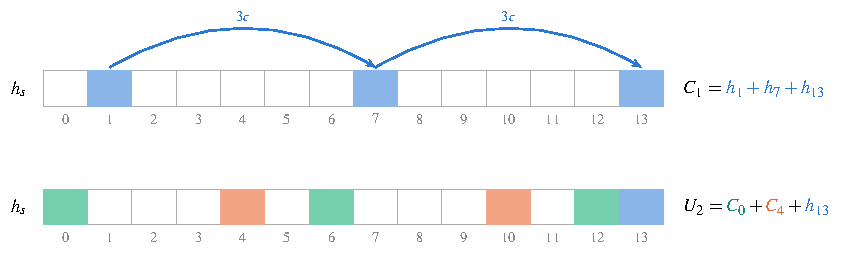
\includegraphics[width=0.8\textwidth]{fig_comb.pdf}
\caption{Comb sums and the closed-form expression
\eqref{eq:Uclosed} for $b=11$, $c=2$
($m=15$, $n=13$, stride $3c=6$).
Top: the comb sum $C_1$, formed by coefficients
at intervals of $6$.
Bottom: $U_2=C_0+C_4+h_{13}$, comprising
two comb sums (green and orange) and one
additional high coefficient (blue).}
\label{fig:comb}
\end{figure*}

% ==================================================================
\section{The closed-form reduction program}\label{sec:program}
% ==================================================================

The closed-form expressions of \cref{thm:quotient} allow intermediate results to
be shared across the reduction circuit. Each comb sum $C_t$ is computed once and
reused in the expressions for $U_k$. These values, in turn, contribute to both
$r_k$ and $r_{k+b}$ whenever the corresponding indices are within range.

Additional sharing is possible for $0\le i\le c-2$. In this range, the
expression $C_i+h_{i+b+c}$ occurs in both $U_i$ and $U_{i+c}$, since
$h_{(i+c)+b}=h_{i+b+c}$. We therefore introduce the intermediate values
$Z_i=C_i\xor h_{i+b+c}$. The resulting reduction procedure is given in
\cref{alg:main}.

\begin{algorithm}[t]
\caption{Reduction modulo $f_{b,c}$, with
$m=b+2c$, $n=m-2$ and $h_s=d_{m+s}$.}
\label{alg:main}
\Input{$d_0,\dots,d_{2m-2}$}
\Output{$r_0,\dots,r_{m-1}$ with
$\sum r_ix^i=D\bmod f_{b,c}$}

\For(\tcp*[f]{comb sums}){$t\gets n$ \KwTo $0$}{
  \lIf{$t+3c\le n$}{
    $C_t\gets h_t\xor C_{t+3c}$
  }
  \lElse{$C_t\gets h_t$}
}

\For(\tcp*[f]{shared pairs}){$i\gets0$ \KwTo $c-2$}{
  $Z_i\gets C_i\xor h_{i+b+c}$
}

\For(\tcp*[f]{values $U_k$}){$k\gets0$ \KwTo $m-1$}{
  \uIf{$k\le c-2$}{
    $U_k\gets Z_k\xor C_{k+c}$
  }
  \uElseIf{$k=c-1$}{
    $U_k\gets C_{c-1}\xor C_{2c-1}$
  }
  \uElseIf{$k\le 2c-2$}{
    $U_k\gets Z_{k-c}\xor C_{k+c}$
  }
  \uElseIf{$k\le b+c-2$}{
    $U_k\gets C_{k-c}\xor C_{k+c}$
  }
  \lElse{$U_k\gets C_{k-c}$}
}

\For(\tcp*[f]{outputs}){$i\gets0$ \KwTo $m-1$}{
  \lIf{$i\ge b$}{
    $r_i\gets (d_i\xor U_i)\xor U_{i-b}$
  }
  \lElse{$r_i\gets d_i\xor U_i$}
}
\end{algorithm}

The algorithm consists of four stages: computing the comb sums, forming the
shared pairs, evaluating the coefficients $U_k$, and constructing the remainder.
Each stage uses values obtained in the preceding stages. All conditional
branches depend only on $b$ and $c$, so fixed parameters determine a
straight-line program of XOR operations.

The comb sums are evaluated in descending order because $C_t$ depends on
$C_{t+3c}$. When $t+3c>n$, the sum contains only $h_t$ and requires no XOR gate.

The computation of $U_k$ is divided into five ranges according to which terms of
\eqref{eq:Uclosed} remain nonzero. The shared values $Z_i$ are used in the first
and third ranges. At $k=c-1$, the additional coefficient $h_{m-1}$ vanishes. For
$k\ge2c-1$, the term $h_{k+b}$ is zero, and for $k\ge b+c-1$, $C_{k+c}$ also
vanishes. In the final range, $U_k=C_{k-c}$ requires no additional XOR
operation.

The remainder coefficients are then obtained from \eqref{eq:rU}. Each output
contains $d_i\xor U_i$, with an additional term $U_{i-b}$ when $i\ge b$.

\begin{theorem}[Main result]\label{thm:main}
For all $b>c\ge1$, \cref{alg:main} computes $D\bmod f_{b,c}$ using at most
$3m-c-3$ XOR gates. Consequently,
\[
  \Red(f_{b,c})\le3m-c-3.
\]
\end{theorem}

\begin{proof}
\emph{Correctness.} The first loop computes the comb sums $C_t$ according to
their definition.

For $0\le k\le c-2$, the shared value $Z_k$ gives
\[
  Z_k+C_{k+c}
  =C_k+C_{k+c}+h_{k+b+c}=U_k,
\]
by \eqref{eq:Uclosed}. At $k=c-1$, the term $h_{k+b+c}=h_{m-1}$ vanishes.

For $c\le k\le2c-2$, we have
\[
  Z_{k-c}+C_{k+c}
  =C_{k-c}+h_{k+b}+C_{k+c}=U_k.
\]
When $2c-1\le k\le b+c-2$, the coefficient $h_{k+b}$ is zero, leaving
$U_k=C_{k-c}+C_{k+c}$. Finally, for $k\ge b+c-1$, $C_{k+c}=0$, so $U_k=C_{k-c}$.
Thus, every branch computes the corresponding expression in \eqref{eq:Uclosed}.

The final loop implements \eqref{eq:rU} and therefore produces the coefficients
of $D\bmod f_{b,c}$.

\emph{XOR count.} The comb sums require one XOR for each index satisfying
$t+3c\le n$. Since $n=b+2c-2$ and $b>c$, their total cost is
\[
  n-3c+1=b-c-1.
\]

The shared pairs $Z_i$ require $c-1$ XOR gates. Computing the values $U_k$
requires one XOR for each $0\le k\le b+c-2$, giving $b+c-1$ gates. No additional
gates are needed for the remaining values.

The output stage requires $m$ XOR gates to compute $d_i\xor U_i$, and another
$m-b=2c$ gates for the outputs containing $U_{i-b}$.

Adding these contributions gives
\begin{align*}
&(b-c-1)+(c-1)+(b+c-1)+m+2c\\
&\qquad=2b+3c-3+m\\
&\qquad=3m-c-3.
\end{align*}
This establishes the stated upper bound. The count assumes that all operands are
distinct. If some of them coincide or cancel, the program becomes shorter, never
longer. In our verification up to $m=1100$, this happens only for the equally
spaced members $b=2c$.
\end{proof}

We verified \cref{alg:main} symbolically for all $201\,117$ members of the family
with $m\le1100$: in every case, the program computes $D\bmod f_{b,c}$ exactly,
as a linear map on the $2m-1$ input coefficients, and uses exactly $3m-c-3$ XOR
gates.

The bound corresponds to fewer than three XOR gates per output bit. For a fixed
degree $m$, increasing $c$ decreases the bound, subject to $b>c$. Members with
small $c$ are the most expensive under this bound; \cref{sec:chains} gives a
construction that favors them. The implications for polynomial selection are
discussed in \cref{sec:comparison}.

Two parameter choices illustrate the gate count. For $b=6$ and $c=5$, the four
stages require $0+4+10+26=40$ gates, matching $3\cdot16-5-3=40$. In this case,
$3c=15>n=14$, so the comb sums require no XOR operations.

For $b=11$ and $c=2$, the respective costs are $8+1+12+19=40$, again matching
$3\cdot15-2-3=40$. Here the comb sums account for eight gates, reflecting the
smaller stride $3c=6$.

\begin{proposition}[Depth]\label{prop:depth}
The XOR depth of \cref{alg:main} is at most
\[
  \left\lfloor\frac{n}{3c}\right\rfloor+4.
\]
In particular, it is at most $5$ when $b\le4c+1$.
\end{proposition}

\begin{proof}
Each comb sum $C_t$ is computed through a chain of $\lfloor(n-t)/(3c)\rfloor$
XOR gates. Hence the maximum depth of this stage is
\[
  \theta=\left\lfloor\frac{n}{3c}\right\rfloor.
\]
The shared values $Z_i$ have depth at most $\theta+1$, and the values $U_k$ have
depth at most $\theta+2$. The final output stage adds at most two XOR levels,
giving a maximum depth of $\theta+4$.

If $b\le4c+1$, then $n=b+2c-2<6c$, so $\theta\le1$. The depth is therefore at
most $5$.
\end{proof}

For the $14\,748$ parameter pairs with $7\le m<300$, the measured depth equals
$\lfloor n/(3c)\rfloor+3$ in $97\%$ of the cases. When $b$ is large relative to
$c$, the longer comb-sum chains become the main source of circuit depth.

A balanced-tree implementation of the comb sums reduces the depth to
$O(\log(n/c))$, at the expense of additional XOR gates (\cref{prop:lowdepth}).

\begin{corollary}[Multiplier]\label{cor:mult}
A schoolbook multiplier for $\F_2[x]/(f_{b,c})$ requires $m^2$ AND gates and at
most
\[
  (m-1)^2+3m-c-3
  =m^2+m-c-2
\]
XOR gates. This is $c+1$ fewer XOR gates than the corresponding bound for
Banegas' first family (\cref{tab:known}).
\end{corollary}

\begin{example}\label{ex:16}
Consider the degree-$16$ pentanomial
\[
  f_{6,5}=x^{16}+x^{11}+x^6+x^5+1.
\]
It is irreducible, whereas no irreducible trinomial exists in degree
$16\equiv0\pmod8$.

Here $n=14$ and $3c=15>n$, so every comb sum consists of a single coefficient,
$C_t=h_t$. The reduction circuit therefore benefits from sharing the pairs $Z_i$
and the values $U_k$, without requiring XOR gates for the comb sums.

\Cref{tab:ex16} gives the resulting program. It uses $40$ XOR gates, compared
with a direct count of $\dX(f)=54$ and a Conta-XOR count of $\CX(f)=44$.
\end{example}

\begin{table*}[t]
\centering\small
\caption{Reduction program for
$f_{6,5}=x^{16}+x^{11}+x^6+x^5+1$
(\cref{ex:16}).}
\label{tab:ex16}
\begin{tabular}{@{}l l l@{}}
\toprule
Step & Instructions & XORs\\
\midrule
Pairs
  & $Z_i=h_i\xor h_{i+11}$, $i=0,\dots,3$
  & 4\\
$U$
  & $U_i=Z_i\xor h_{i+5}$ ($i\le3$);
    $U_4=h_4\xor h_9$
  & 5\\
  & $U_i=Z_{i-5}\xor h_{i+5}$ ($5\le i\le8$);
    $U_9=h_4\xor h_{14}$
  & 5\\
  & $U_i=h_{i-5}$ for $10\le i\le15$
  & 0\\
Outputs
  & $r_i=d_i\xor U_i$ ($0\le i\le5$);
    $r_i=d_i\xor U_i\xor U_{i-6}$ ($6\le i\le15$)
  & 26\\
\midrule
Total & & $40=3m-c-3$\\
\bottomrule
\end{tabular}
\end{table*}


% ==================================================================
\section{A shorter program from the chain structure}\label{sec:chains}
% ==================================================================

\Cref{alg:main} is a direct transcription of the closed form, and it is not
optimal. Exact minima computed with a SAT solver (\cref{tab:exact}) lie below
$3m-c-3$ for every small generic member we could solve. In this section we show
where the slack comes from and remove most of it for $b\ge4c+1$.

In the middle range of \eqref{eq:Uclosed}, \cref{alg:main} spends about two
gates per value $U_k$: one to extend a comb sum and one to add two comb sums.
The comb sums themselves, however, are never needed. Only the sums
\begin{align*}
  E_t&=C_t+C_{t+c}, && t\ge0,\\
  P_k&=C_{k-c}+C_{k+c}, && k\ge c
\end{align*}
appear in \eqref{eq:Uclosed}: $U_k=E_k+h_{k+b+c}$ for $k<c$, and $U_k=P_k$ for
$2c-1\le k\le b+c-2$. These sums can be obtained from each other directly.

\begin{lemma}[Chain identities]\label{lem:chain}
For all $t\ge0$ and $k\ge c$,
\begin{enumerate}[label=(\roman*),itemsep=1pt]
  \item $E_t=h_t+P_{t+2c}$;
  \item $P_k=h_{k-c}+E_{k+c}$;
  \item $P_k=E_{k-c}+E_k$.
\end{enumerate}
Moreover, $E_t=h_t$ for $t>n-c$, and $P_k=h_{k-c}$ for $k>n-c$.
\end{lemma}

\begin{proof}
(i) Since $C_t=h_t+C_{t+3c}$, we get
$E_t=h_t+C_{t+c}+C_{t+3c}=h_t+P_{t+2c}$.
(ii) Similarly, $C_{k-c}=h_{k-c}+C_{k+2c}$ gives
$P_k=h_{k-c}+C_{k+c}+C_{k+2c}=h_{k-c}+E_{k+c}$.
(iii) The two occurrences of $C_k$ cancel.
If $t>n-c$, then $C_{t+c}=0$ and, since $t+3c>n$, $C_t=h_t$. If $k>n-c$, then
$C_{k+c}=0$ and, since $k+2c>n$, $C_{k-c}=h_{k-c}$.
\end{proof}

Identities (i) and (ii) cost one gate each and alternate between the two kinds
of sums: starting from the top, $P_k$ gives $E_{k-2c}$, which gives
$P_{k-3c}$, and so on. Such a \emph{strand} produces one value $E$ and one value
$P$ every $3c$ positions, at one gate each, and needs no comb sum. All shifts
are multiples of $c$, so the computation splits into $c$ independent
\emph{chains}, one for each residue class of the index modulo $c$. Within a
chain, consecutive indices differ by $c$, and we group them in blocks of three.
Two strands per chain provide $E$ at two of every three positions and $P$ at two
of every three positions. The remaining value $P$ comes from (iii), at one more
gate. The cost is therefore five gates per three positions, instead of the six
gates of \cref{alg:main}.

To state precisely which values are computed, let
\[
  \sigma(t)=\left\lfloor\frac{t+1}{c}\right\rfloor\bmod 3 .
\]
Since $\sigma(t+c)\equiv\sigma(t)+1\pmod3$, the value of $\sigma$ advances by one
along each chain. The program, given in \cref{alg:chain}, computes $E_t$ when
$\sigma(t)\neq2$, obtains $P_k$ from a strand when $\sigma(k)\ne1$, and uses
(iii) when $\sigma(k)=1$. Values with index above $n-c$ are taken from the
last part of \cref{lem:chain} and cost nothing. The values $U_k$ with $c\le k\le
2c-2$ use $U_k=U_{k-c}+E_k$, which replaces the shared pairs $Z_i$ of
\cref{alg:main}.

\begin{algorithm}[t]
\caption{Chain construction for reduction modulo $f_{b,c}$, with $m=b+2c$,
$n=m-2$, $h_s=d_{m+s}$, and $E_t=h_t$, $P_k=h_{k-c}$ for indices above $n-c$.}
\label{alg:chain}
\Input{$d_0,\dots,d_{2m-2}$}
\Output{$r_0,\dots,r_{m-1}$ with
$\sum r_ix^i=D\bmod f_{b,c}$}

\For(\tcp*[f]{strands}){$i\gets n-c$ \KwTo $0$}{
  \lIf{$i\ge2c-1$ \KwAnd $\sigma(i)\ne1$}{
    $P_i\gets h_{i-c}\xor E_{i+c}$
  }
  \lIf{$\sigma(i)\ne2$}{
    $E_i\gets h_i\xor P_{i+2c}$
  }
}

\For(\tcp*[f]{third values}){$k\gets 2c-1$ \KwTo $n-c$}{
  \lIf{$\sigma(k)=1$}{
    $P_k\gets E_{k-c}\xor E_k$
  }
}

\For(\tcp*[f]{values $U_k$}){$k\gets0$ \KwTo $m-1$}{
  \uIf{$k\le c-2$}{
    $U_k\gets E_k\xor h_{k+b+c}$
  }
  \uElseIf{$k=c-1$}{
    $U_k\gets E_{c-1}$
  }
  \uElseIf{$k\le 2c-2$}{
    $U_k\gets U_{k-c}\xor E_k$
  }
  \uElseIf{$k\le b+c-2$}{
    $U_k\gets P_k$
  }
  \lElse{$U_k\gets h_{k-c}$}
}

\For(\tcp*[f]{outputs}){$i\gets0$ \KwTo $m-1$}{
  \lIf{$i\ge b$}{
    $r_i\gets (d_i\xor U_i)\xor U_{i-b}$
  }
  \lElse{$r_i\gets d_i\xor U_i$}
}
\end{algorithm}

\begin{theorem}[Chain construction]\label{thm:chain}
For all $b>c\ge1$, \cref{alg:chain} computes $D\bmod f_{b,c}$ using exactly
$3m-3-N(b,c)$ XOR gates, where $u$ ranges over the positive integers and
\begin{align*}
  N(b,c)&=\#\bigl\{u\le b+c-1:\
          \lfloor u/c\rfloor\equiv2\!\!\pmod 3\bigr\}\\
        &=c\left\lfloor\frac{b+c}{3c}\right\rfloor\\
        &\qquad+\max\bigl(0,\,((b+c)\bmod 3c)-2c\bigr).
\end{align*}
Consequently,
\[
  \Red(f_{b,c})\le\min\bigl\{3m-c-3,\ 3m-3-N(b,c)\bigr\}.
\]
The second bound is larger than the first when $b<2c$, equal to it when
$2c\le b\le4c$, and smaller by $N(b,c)-c\ge1$ when $b\ge4c+1$. In all cases
$3m-3-N(b,c)\le\tfrac83m+c-3$.
\end{theorem}

\begin{proof}
\emph{Availability of operands.} In the first loop, $P_i$ with $\sigma(i)\ne1$
uses $E_{i+c}$. Either $i+c>n-c$, and the value is free by \cref{lem:chain}, or
$\sigma(i+c)=\sigma(i)+1\in\{0,1\}$ and $E_{i+c}$ was computed at the earlier
step $i+c$. Likewise, $E_i$ with $\sigma(i)\ne2$ uses $P_{i+2c}$, which is
either free or has $\sigma(i+2c)=\sigma(i)+2\in\{0,2\}$ and index at least
$2c-1$, so it was computed at step $i+2c$. In the second loop, $\sigma(k)=1$
gives $\sigma(k-c)=0$, so both $E_{k-c}$ and $E_k$ are available. The values
$E_k$ with $k\le 2c-2$ used in the third loop have $\sigma(k)\in\{0,1\}$.

\emph{Correctness.} By \cref{lem:chain}, every gate of the first two loops
computes the value it names. For the values $U_k$ we use \eqref{eq:Uclosed}.
If $k\le c-2$, then $U_k=C_k+C_{k+c}+h_{k+b+c}=E_k+h_{k+b+c}$. At $k=c-1$,
$h_{m-1}=0$ and $U_{c-1}=E_{c-1}$. If $c\le k\le 2c-2$, then
\begin{align*}
  U_k&=C_{k-c}+C_{k+c}+h_{k+b}\\
     &=(E_{k-c}+h_{k+b})+E_k
      =U_{k-c}+E_k .
\end{align*}
If $2c-1\le k\le b+c-2$, then $k+b>n$ and $U_k=P_k$; for larger $k$,
$U_k=C_{k-c}=h_{k-c}$ as in \cref{alg:main}. The last loop is \eqref{eq:rU}.

\emph{XOR count.} The values $P_k$ with $2c-1\le k\le n-c$ cost one gate each,
in the first or in the second loop, which gives $n-3c+2=b-c$ gates. The values
$E_t$ with $0\le t\le n-c$ and $\sigma(t)\ne2$ cost one gate each; with $u=t+1$,
the excluded indices are exactly those counted by $N(b,c)$, so this gives
$b+c-1-N(b,c)$ gates. The values $U_k$ cost $2(c-1)$ gates, and the outputs
cost $m+2c$, as in \cref{thm:main}. The total is
\[
  (b-c)+(b+c-1-N)+2c-2+m+2c=3m-3-N(b,c).
\]

\emph{The count $N(b,c)$.} The integers $u$ with $\lfloor u/c\rfloor\equiv2
\pmod3$ form the blocks $[2c,3c-1]$, $[5c,6c-1]$, and so on, of $c$ integers
each. Writing $b+c=3c\eta+\xi$ with $0\le\xi<3c$, the range $1\le u\le b+c-1$
contains $\eta$ complete blocks and $\max(0,\xi-2c)$ elements of the next one.
If $b<2c$, then $b+c-1<3c-1$ and $N=b-c<c$. If $2c\le b\le4c$, the first
block is complete and the second is not reached, so $N=c$. If $b\ge4c+1$, then
$b+c-1\ge5c$ and $N\ge c+1$. Finally, $N\ge(b+c-2c)/3=(b-c)/3$, and
$b-c=m-3c$ gives $3m-3-N\le\tfrac83m+c-3$.
\end{proof}

With a schoolbook multiplier, \cref{thm:chain} gives $m^2+m-2-N(b,c)$ XOR
gates. For $c=1$ the bound becomes $3m-3-\lfloor(m-1)/3\rfloor\approx\tfrac83m$, so
members with small $c$, which were the most expensive under \cref{thm:main},
now reach the same asymptotic cost as members with $c$ close to $m/3$. For a
fixed degree, the better of the two bounds is close to $\tfrac83m$ at both ends
of the range of $c$ and largest, about $\tfrac{17}6m$, near $b=4c$.

We verified \cref{alg:chain} symbolically for all $201\,117$ members with
$m\le1100$: it computes $D\bmod f_{b,c}$ exactly and uses exactly
$3m-3-N(b,c)$ gates. It improves on \cref{thm:main} for $100\,284$ of them.
The construction also explains several entries of \cref{tab:exact}. For
$f_{6,1}$ it gives $19$ gates, which is optimal, and for $f_{5,1}$ it gives
$16$, the optimum of \cref{tab:base}. For $f_{7,1}$, $f_{8,1}$ and $f_{9,1}$ it
gives $22$, $24$ and $27$ gates, the best values that the SAT solver found.
For members with $2c\le b\le4c$, such as $f_{5,2}$, the SAT solver still finds
one gate less, so some slack remains in that range.

\begin{example}\label{ex:chain}
For $f_{8,1}=x^{10}+x^9+x^8+x+1$ we have $m=10$, $n=8$, $c=1$ and
$\sigma(t)=(t+1)\bmod3$. \Cref{alg:chain} computes
\begin{align*}
  P_7&=h_6\xor h_8, & E_6&=h_6\xor h_7,\\
  P_5&=h_4\xor E_6, & E_5&=h_5\xor P_7,\\
  P_4&=h_3\xor E_5, & E_3&=h_3\xor P_5,\\
  P_2&=h_1\xor E_3, & E_2&=h_2\xor P_4,\\
  P_1&=h_0\xor E_2, & E_0&=h_0\xor P_2,\\
  P_3&=E_2\xor E_3, & P_6&=E_5\xor E_6,
\end{align*}
and then $U_0=E_0$, $U_k=P_k$ for $1\le k\le7$, $U_8=h_7$ and $U_9=h_8$. These
are $12$ gates, against $14$ in \cref{alg:main} (six for the comb sums and
eight for the values $U_k$). With the $12$ output gates, the total is
$24=3m-3-N(8,1)$, compared with $3m-c-3=26$.
\end{example}

The gain has a price in depth. Along a strand, each step of $3c$ positions adds
two levels instead of one.

\begin{proposition}[Depth of the chain construction]\label{prop:chaindepth}
The XOR depth of \cref{alg:chain} is at most
$2\lfloor(n-c)/(3c)\rfloor+6$.
\end{proposition}

\begin{proof}
By induction from the top, the value $E_t$ has depth at most
$2\lfloor(n-c-t)/(3c)\rfloor+2$, since $E_t$ depends on $P_{t+2c}$, which
depends on $E_{t+3c}$. Hence every value $E_t$ has depth at most
$\Delta=2\lfloor(n-c)/(3c)\rfloor+2$, every value $P_k$ and every $U_k$ with
$k\le c-2$ has depth at most $\Delta+1$, and every $U_k$ with $c\le k\le 2c-2$
has depth at most $\Delta+2$. The outputs add two more levels.
\end{proof}

In our verification up to $m=1100$, the depth never exceeded
$2\lfloor(n-c)/(3c)\rfloor+5$. For the NIST-degree member
$x^{571}+x^{549}+x^{527}+x^{22}+1$, \cref{alg:chain} uses $1534$ gates and has
depth $20$, against $1688$ gates and depth $11$ for \cref{alg:main}. The two
constructions therefore offer a trade-off between area and delay. The
word-level formulation and the low-depth variant of the next section are based
on \cref{alg:main}.

The construction is also optimal in a restricted sense. We modeled one chain as
a weighted MaxSAT problem whose programs may use the comb sums, the values $E$
and $P$, the shared pairs $Z_i$, and every identity of \cref{lem:chain} and
\cref{thm:quotient}. For every chain length up to $1100$, the optimum equals
the cost of \cref{alg:chain}, except for the shortest chains, with three
indices, where the shared pairs of \cref{alg:main} save one gate; such chains
occur only when $b<2c$. Shorter programs, such as the one for $f_{5,2}$, must
therefore use sums that are not of the forms considered here.


% ==================================================================
\section{Word-level formulation and a low-depth variant}\label{sec:word}
% ==================================================================

The closed-form quotient of \cref{thm:quotient} can also be expressed using
shifts and XOR operations on bit vectors. This formulation is suitable for
software implementations, where several polynomial coefficients can be processed
simultaneously. Throughout the section we work with \cref{alg:main}; the chain
construction of \cref{sec:chains} has a longer critical path, and we do not
pursue a word-level form of it.

We represent a polynomial by a bit vector whose bit $i$ is the coefficient of
$x^i$. The notation $A\gg k$ denotes a right shift by $k$ positions,
corresponding to $\lfloor A/x^k\rfloor$, while $A\ll k$ denotes multiplication
by $x^k$.

\begin{corollary}[Word-level reduction]
\label{cor:word}
With $L$ and $H$ as defined in \eqref{eq:split}, let
\begin{align*}
  C &= \textstyle\sum_{\ell\ge0}(H\gg 3c\ell),\\
  Q &= C\xor(C\gg c)\xor(H\gg(b+c)),\\
  U &= Q\xor(Q\ll c).
\end{align*}
Then
\[
  D\bmod f_{b,c}
  =\bigl(L\xor U\xor(U\ll b)\bigr)\bmod x^m.
\]
The vector $C$ can be computed by initializing $C\gets H$ and applying
\[
  C\gets C\xor(C\gg 3c\cdot2^j)
\]
for successive integers $j\ge0$ such that $3c\cdot2^j\le n$.
\end{corollary}

\begin{proof}
The coefficient of $x^t$ in $\sum_{\ell\ge0}(H\gg3c\ell)$ is the comb sum $C_t$. The
expression for $Q$ follows from \eqref{eq:qclosed}, while $U=(1+x^c)Q$ and the
expression for the remainder follow from \eqref{eq:rU}.

After doubling step $j$, each coefficient of $C$ contains the sum of the
corresponding $2^{j+1}$ terms, or all available terms if fewer remain. Thus, the
complete comb sums are obtained once $3c\cdot2^{j+1}>n$.
\end{proof}

The vector formulation evaluates all comb sums through a sequence of shifts and
XOR operations. The correction term $H\gg(b+c)$ can have nonzero coefficients
only at positions $j\le c-2$. In the final expression, reduction modulo $x^m$
amounts to discarding bits above position $m-1$.

The doubling procedure avoids computing each shifted copy of $H$ separately. At
each step, the number of terms accumulated in each position doubles. For
example, with $b=7$ and $c=1$, we have $n=7$ and stride $3$. The first step
combines $h_t$ and $h_{t+3}$, while the second includes $h_{t+6}$ and $h_{t+9}$,
with out-of-range coefficients taken as zero.

Let
\[
  \nu=\left\lceil
  \log_2\left(\frac{n+1}{3c}\right)
  \right\rceil,
\]
with $\nu=0$ when $3c>n$. The reduction requires $\nu+5$ shift-and-XOR operations on
bit vectors: $\nu$ for the comb sums, two for $Q$, one for $U$, and two for the
remainder. Hence the number of vector operations grows logarithmically with
$m/c$.

This count assumes operations on complete bit vectors and does not directly
represent the number of machine instructions. The latter depends on the
processor architecture, register width and representation of the field elements.

When $b\le4c+1$, we have $\nu\le1$, and the reduction requires at most six
shift-and-XOR operations. This includes the selected members of degrees $163$
and $571$ discussed in \cref{sec:comparison}. The formulation can be used after
carry-less polynomial multiplication, for example with \texttt{PCLMULQDQ}, or in
bitsliced implementations.

The same doubling procedure can be applied at the gate level to reduce the depth
of the comb-sum computation.

\begin{proposition}[Low-depth variant]
\label{prop:lowdepth}
Replacing the sequential comb sums in \cref{alg:main} with the doubling
procedure of \cref{cor:word} gives a reduction circuit with at most
\[
  3m-c-3+
  \sum_{j=1}^{\nu-1}
  \max\bigl(0,\,
  n+1-3c\cdot2^j\bigr)
\]
XOR gates and depth at most $\nu+4$.
\end{proposition}

\begin{proof}
At doubling step $j$, an XOR gate is required for each position $t$ satisfying
$t+3c\cdot2^j\le n$. The number of gates at that step is therefore
\[
  \max(0,n+1-3c\cdot2^j).
\]
Each step adds one level to the circuit depth.

The first step, $j=0$, requires $n+1-3c=b-c-1$ gates, matching the comb-sum cost
in \cref{alg:main}. The remaining steps account for the additional gates in the
stated bound.

The subsequent stages are unchanged and contribute at most four levels, as
established in \cref{prop:depth}. Thus, the overall depth is at most $\nu+4$.
\end{proof}

The two implementations provide different trade-offs between gate count and
circuit depth. In \cref{alg:main}, each comb sum is computed sequentially from
the preceding one. A sum containing $d$ terms therefore requires a chain of
$d-1$ dependent XOR gates.

The doubling procedure combines partial sums in parallel, reducing the depth to
$\lceil\log_2d\rceil$, although additional gates may be required. When
$b\le4c+1$, each comb sum contains at most two terms, and the two constructions
coincide. The low-depth variant is therefore most relevant when $c$ is small
relative to $m$.

We verified the low-depth variant symbolically for all members with $m\le1100$,
including its gate count and depth bound. As
an illustration, consider
\[
  f=x^{571}+x^{549}
    +x^{527}+x^{22}+1,
\]
where $b=527$, $c=22$, $n=569$ and the stride is $66$.

The comb sums contain up to nine terms, giving $\nu=4$. The sequential
construction of \cref{alg:main} has depth $11$ and uses $1688$ XOR gates. The
doubling variant reduces the depth to $7$ but requires $2474$ gates.

Thus, the reduction of four depth levels comes at the cost of $786$ additional
XOR gates, an increase of approximately $47\%$. The choice between the two
constructions depends on the area and delay requirements of the implementation.


% ==================================================================
\section{Comparison with the greedy count}\label{sec:greedy}
% ==================================================================

Banegas' second family was originally identified using Conta-XOR
\cite{Banegas2015}. We compare the reduction costs obtained from the closed-form
construction with those produced by this heuristic. The analysis follows the
classification introduced in \cref{def:special}: members with
$b/c\in\{\tfrac32,2,3,4,5\}$ are considered special, while all others are
generic.

\begin{observation}\label{obs:greedy}
We evaluated $\CX(f_{b,c})$ for all $3\,674$ parameter pairs with $5\le
m\le150$. For each pair, we also performed $20$ additional greedy runs with
randomized tie-breaking, following the approach of \cite{TanPeyrin2020}.

Among the $3\,541$ generic members, we observed the following:
\begin{enumerate}[label=(\alph*),itemsep=1pt]
  \item The closed-form construction was
  never more expensive than either greedy result.

  \item For all $879$ members with $b<2c$,
  $\CX(f)=2m+3c-3$. The closed-form construction therefore used exactly $2c-b$
  fewer XOR gates.

  \item For all $1\,312$ members satisfying
  $2c<b<6c$, the greedy count was $\CX(f)=3m-c-3$, equal to the closed-form
  count.

  \item For $b\ge6c$, the greedy count
  exceeded the closed-form count in $392$ of the $1\,350$ cases, with
  differences of up to $112$ XOR gates.
\end{enumerate}

Randomized tie-breaking improved the greedy count for $212$ generic members, all
with $b\ge6c$, by at most $12$ gates. In only one of these cases did the
improvement eliminate the difference relative to the closed-form construction.
These figures depend on the random choices; an independent rerun gave $213$
members and at most $13$ gates, again all with $b\ge6c$ and with a single case
closing the gap.

For special members, the greedy counts follow the strip bound
\eqref{eq:specialbound}, with the values of $R_1(G)$ and $R_2(G)$ that the
greedy algorithm finds for each base polynomial. For $f_{2,1}$ and $f_{3,1}$ these are the
optimal values of \cref{tab:base}; for $f_{4,1}$, $f_{5,1}$ and $f_{3,2}$ the
lexicographic greedy algorithm finds programs one or two gates longer
($R_1=16$ for $f_{4,1}$, and $R_2=17$, $R_1=19$ for $f_{5,1}$ and $f_{3,2}$). For example, when
$b=3c$, the observed cost was $\tfrac{12}{5}m-2$ XOR gates. Since the reduction matrix of
$f$ is block diagonal over the strips (\cref{rem:strips}), the greedy algorithm
never mixes strips and effectively reduces modulo $G$ once per strip.
\end{observation}

The results indicate that randomized tie-breaking has limited influence on the
differences observed between the two constructions. This suggests that the
choice of intermediate expressions, rather than tie-breaking alone, may account
for part of the difference. The experiments do not, however, establish that the
closed-form counts are optimal.

\Cref{fig:gain} shows $\CX(f)-(3m-c-3)$ as a function of $b/c$, using a
logarithmic horizontal scale. The figure includes all generic members with
$m\le150$. Every difference is nonnegative, and three regions can be
distinguished.

For $b/c<2$, the difference is exactly
\[
  2c-b=c(2-b/c).
\]
At a fixed ratio, the difference increases with $c$ and therefore with the field
degree. The largest difference in this region is $48$ gates, obtained for
$b=c+1$ and $c=49$.

For $2<b/c<6$, both methods produce programs with the same XOR count. When
$b/c\ge6$, the greedy algorithm produces larger counts for some members,
particularly when $c$ is small. In these cases, the comb sums contain more
terms, and the ordering of intermediate XOR operations becomes increasingly
relevant. The curves extending toward larger ratios correspond to fixed small
values of $c$, such as $c=1$ and $c=2$, with increasing $m$.

The same regularities hold beyond the range of \cref{obs:greedy}. We ran the
greedy algorithm, with lexicographic tie-breaking, on all $11\,175$ members with
$151\le m\le300$ and on all members of degrees $500$, $800$ and $1100$. For every
generic member, the closed form was never more expensive; the greedy count was
exactly $2m+3c-3$ when $b<2c$ and exactly $3m-c-3$ when $2c<b<6c$. For $b\ge6c$,
the greedy algorithm needed more gates in $598$ of the $4\,163$ members with
$151\le m\le300$ and in $36$ of the $299$ members of the three larger degrees, by
up to $248$ and $994$ XOR gates, respectively. The fraction of such members
decreases as $m$ grows, but the excess, when it occurs, becomes larger.

The same comparison can be made for the polynomials reported in Banegas' thesis.
\Cref{tab:thesis} lists the irreducible members of the second family at the NIST
field degrees, including those reported in \cite[Tab.~17]{Banegas2015}.

For the listed members with $b>2c$, the greedy counts coincide with $3m-c-3$.
When $b<2c$, the closed-form construction requires fewer gates. The two listed
members with $b\ge4c+1$ are improved by the chain construction: the degree-$233$
member with $c=16$ needs $632$ gates instead of $680$, and the degree-$571$
member with $c=22$ needs $1534$ instead of $1688$. Neither changes the best
member of its degree.

For example,
\[
  f=x^{163}+x^{117}+x^{71}+x^{46}+1
\]
has $b=71$ and $c=46$. Its greedy count is $461$, whereas the closed-form
construction requires $440$ gates, a reduction of $21=2\cdot46-71$ XOR gates.

\begin{figure*}[t]
\centering
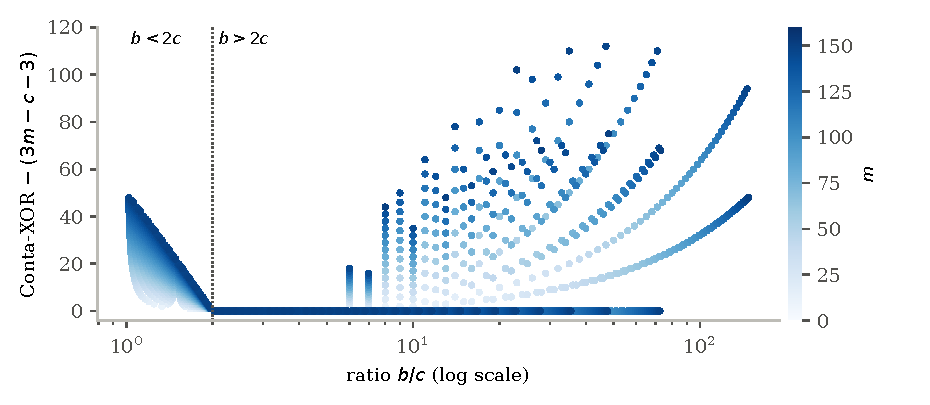
\includegraphics[width=0.85\textwidth]{fig_gain.pdf}
\caption{Difference between the Conta-XOR
count and the closed-form count,
$\CX(f)-(3m-c-3)$, for the $3\,541$
generic members with $m\le150$.
Color indicates the degree $m$,
and the dotted line marks $b/c=2$.
The difference is nonnegative
throughout the evaluated range.
For $b/c<2$, it equals $2c-b$;
for $2<b/c<6$, it is zero.
Larger differences occur for
some members with $b/c\ge6$.}
\label{fig:gain}
\end{figure*}

\begin{table*}[t]
\centering\small
\caption{Irreducible members of the
second family at the NIST field degrees.
The label ``thesis'' identifies values
reported in \cite[Tab.~17]{Banegas2015}. The depth refers to \cref{alg:main};
the last column is the cost of the chain construction (\cref{thm:chain}).}
\label{tab:thesis}
\begin{tabular}{@{}r l r r r r r r r@{}}
\toprule
$m$ & $f$ & $b$ & $c$ & $\dX$ & $\CX$ & $3m-c-3$ & depth & $3m-3-N$\\
\midrule
163 & $x^{163}+x^{117}+x^{71}+x^{46}+1$ & 71 & 46 & 649 & 461 & \textbf{440} & 4 & 461\\
233 & $x^{233}+x^{158}+x^{83}+x^{75}+1$ & 83 & 75 & 866 & 688 & \textbf{621} & 4 & 688\\
233 & $x^{233}+x^{217}+x^{201}+x^{16}+1$ & 201 & 16 & 1687 & 680 & 680 & 7 & \textbf{632}\\
409 & $x^{409}+x^{294}+x^{179}+x^{115}+1$ & 179 & 115 & 1642 & 1160 & \textbf{1109} & 4 & 1160\\
409 & $x^{409}+x^{337}+x^{265}+x^{72}+1$ & 265 & 72 & 1823 & 1152 & 1152 & 4 & 1152\\
571 & $x^{571}+x^{389}+x^{207}+x^{182}+1$ & 207 & 182 & 2145 & 1685 (thesis) & \textbf{1528} & 4 & 1685\\
571 & $x^{571}+x^{465}+x^{359}+x^{106}+1$ & 359 & 106 & 2531 & 1604 (thesis) & 1604 & 4 & 1604\\
571 & $x^{571}+x^{549}+x^{527}+x^{22}+1$ & 527 & 22 & 6297 & 1688 (thesis) & 1688 & 11 & \textbf{1534}\\
\bottomrule
\end{tabular}
\end{table*}

We also compared the closed-form construction with the heuristic of Boyar and
Peralta \cite{BoyarPeralta2010}, which can exploit cancellations between
intermediate expressions.

For the generic degree-$9$ and degree-$10$ members, $f_{5,2}$ and $f_{4,3}$, the
best of $10$ runs produced programs with $22$ and $24$ XOR gates, respectively.
Both counts match $3m-c-3$, whereas Conta-XOR gave $22$ and $26$.

For the degree-$7$ special member $f_{3,2}$, both the closed-form construction
and the Boyar and Peralta heuristic required $16$ gates, compared with $17$ for
Conta-XOR.

The closed-form derivation also uses cancellations, notably the elimination of
$C_k$ in $U_k=q_k+q_{k-c}$. Unlike the heuristics, however, \cref{alg:main}
incorporates these cancellations directly into its expressions, without
searching for intermediate XOR combinations.

\paragraph*{Exact minima for small members}
To find out how far the closed form is from optimal, we computed exact minima
with a SAT solver, using the encoding of \cite{Stoffelen2016}. The search is made
feasible by a simple reduction: each low input $d_i$, $i<m$, appears only in the
output $r_i$, so setting it to zero removes at least one gate, and therefore
$\Red(f)=m+\Red(R')$, where $R'$ is the reduction matrix restricted to the high
inputs. \Cref{tab:exact} summarizes the results. For the base polynomials of
\cref{def:special}, the values of \cref{tab:base} are optimal. For every small
generic member we could solve, however, the optimum lies at least one gate below
the closed form, and for $c=1$ the known gap grows with $b$. Neither the greedy algorithm,
with up to $500$ randomized runs, nor the heuristic of Boyar and Peralta finds
these programs. The bound of \cref{thm:main} is therefore not optimal in general.
The chain construction of \cref{sec:chains} attains the optimum for $f_{6,1}$
and $f_{5,1}$, and the best values found by the SAT solver for $f_{7,1}$,
$f_{8,1}$ and $f_{9,1}$. For $f_{5,2}$ and $f_{7,2}$, which satisfy $2c\le
b\le4c$, a gap of one gate remains.

\begin{table}[t]
\centering\small
\caption{Exact minima $\Red(f)$ for small members, computed with a SAT solver,
compared with the closed form, with the best bound of \cref{thm:main,thm:chain}, and
with the best heuristic result (greedy with randomized ties, or Boyar and Peralta). An entry ``$\le v$'' means that a program with $v$ gates exists and that smaller
values were not decided.}
\label{tab:exact}
\setlength{\tabcolsep}{4pt}
\begin{tabular}{@{}l r r r r l@{}}
\toprule
$f$ & $m$ & $3m-c-3$ & best bound & heuristic & $\Red(f)$\\
\midrule
$f_{2,1}$ (special) & $4$ & $8$ & $8$ & $6$ & $6$\\
$f_{3,1}$ (special) & $5$ & $11$ & $11$ & $10$ & $10$\\
$f_{4,1}$ (special) & $6$ & $14$ & $14$ & $14$ & $14$\\
$f_{5,1}$ (special) & $7$ & $17$ & $16$ & $16$ & $16$\\
$f_{3,2}$ (special) & $7$ & $16$ & $16$ & $16$ & $16$\\
$f_{6,1}$ & $8$ & $20$ & $19$ & $20$ & $19$\\
$f_{5,2}$ & $9$ & $22$ & $22$ & $22$ & $21$\\
$f_{7,1}$ & $9$ & $23$ & $22$ & $23$ & $\le22$\\
$f_{8,1}$ & $10$ & $26$ & $24$ & $26$ & $\le24$\\
$f_{7,2}$ & $11$ & $28$ & $28$ & $28$ & $\le27$\\
$f_{9,1}$ & $11$ & $29$ & $27$ & $29$ & $\le27$\\
\bottomrule
\end{tabular}
\end{table}

% ==================================================================
\section{Comparison with the first family and with other polynomials}\label{sec:comparison}
% ==================================================================

\subsection{Parameter selection}

The bound of \cref{thm:main} decreases as $c$ increases, while the bound of
\cref{thm:chain}, which matters when $b\ge4c+1$, grows roughly as
$\tfrac83m+\tfrac13c$. For a fixed degree, the better of the two is therefore
smallest at the two ends of the range of $c$, where it approaches $\tfrac83m$,
and largest near $b=4c$, where it is about $\tfrac{17}6m$. Special members can
do better (\cref{tab:base}), but they exist only in degrees divisible by $4$,
$5$, $6$ or $7$, and they are irreducible only in the few degrees described by
\cref{prop:specirr}. For a given field degree, the best choice is the
irreducible member that minimizes $\min\{3m-c-3,\,3m-3-N(b,c)\}$, and it usually
has $c$ either close to $m/3$ or very small.

For Banegas' first family, the corresponding bound is $3m-2$, independently of
$b$ and $c$, except for the case $m=5c$. Thus, when comparing the
general bounds at the same degree, the second family offers a reduction of at
least $c+1$ XOR gates.

\subsection{Irreducibility census}

We tested all members of both families, as well as all trinomials, for
irreducibility in degrees $5\le m\le1100$, using Rabin's test \cite{Rabin1980}.
The results are summarized in \cref{tab:census}.

Whenever an irreducible trinomial exists, its known reduction cost of $2m-2$ XOR
gates is lower than the general bounds considered here for the two pentanomial
families. We therefore focus on the $502$ degrees in the evaluated range for
which no irreducible trinomial exists.

For these degrees, \cref{fig:census} compares the reduction cost per bit,
defined as the number of XOR gates divided by $m$, for the lowest-cost
irreducible members identified in each family.

For the first family, the general bound gives $3-2/m$ gates per bit, apart from
the case $b=2c$. This value approaches $3$ as $m$ increases.

For the second family, the corresponding expression is the smaller of
\[
  3-\frac{c+3}{m}
  \quad\text{and}\quad
  3-\frac{N(b,c)+3}{m}.
\]
The first approaches $\tfrac83$ when $c$ is close to $m/3$, and the second when
$c$ is small. Across the evaluated degrees, the mean cost per bit of the best
generic member is $2.70$, against $2.77$ with \cref{thm:main} alone. The chain
construction lowers the cost of the best member of the second family in $379$
of the $720$ degrees, $160$ of them without irreducible trinomials, by up to
$11.1\%$. For example, at $m=975$ the member with $c=1$ needs $2598$ XOR gates
instead of $2921$.

\begin{table*}[t]
\centering\small
\caption{Irreducibility census for
$5\le m\le1100$ ($1\,096$ degrees).
The comparison uses the better of \cref{thm:main,thm:chain}
for generic members of the second family
and the strip bound \eqref{eq:specialbound}
with \cref{tab:base} for special members,
and $3m-2$ or $\tfrac{12}{5}m-1$ for the
first family \cite{BCP2019}.}
\label{tab:census}
\begin{tabular}{@{}l r@{}}
\toprule
irreducible members of the second family & $1\,508$\\
degrees with at least one member: second family / first family & $720$ / $502$\\
degrees with members of both families & $405$\\
\quad of which the second family is cheaper & $405$ (mean saving $9.7\%$)\\
degrees in which \cref{thm:chain} improves the best member & $379$\\
degrees without irreducible trinomials & $502$\\
\quad covered by the second family / by the first family & $288$ / $229$\\
\quad covered by the second family only & $112$\\
\quad covered by neither & $161$\\
mean cost per bit of the best generic member of the second family & $2.70$\\
\quad the same with \cref{thm:main} only & $2.77$\\
\bottomrule
\end{tabular}
\end{table*}

\begin{figure*}[t]
\centering
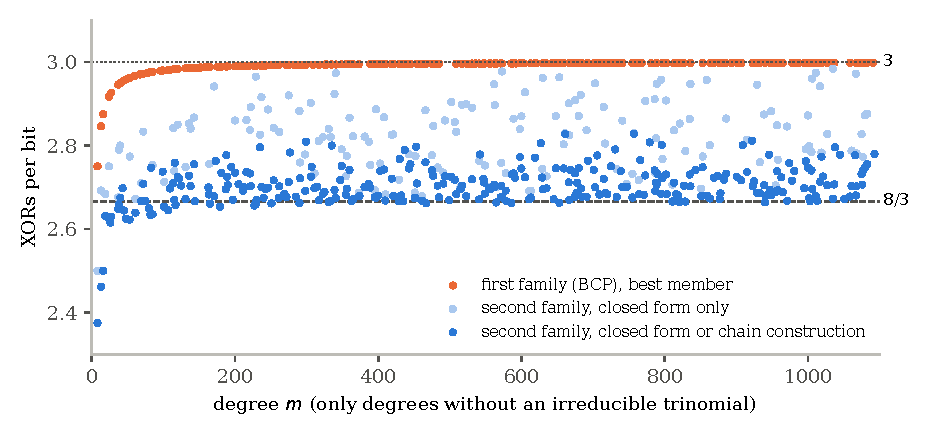
\includegraphics[width=0.85\textwidth]{fig_census.pdf}
\caption{Reduction cost per bit
for degrees $m\le1100$ without
irreducible trinomials.
The figure compares the lowest
reported bounds for members of
Banegas' first family (BCP)
and the second family, with
\cref{thm:main} alone and with
the better of \cref{thm:main,thm:chain}.
The dashed line indicates
the asymptotic limit
$\tfrac83$ of both general
bounds for the second family.}
\label{fig:census}
\end{figure*}

Among the $405$ degrees containing irreducible members of both families, the
second family has a lower reduction bound in all of them, with a mean saving of
$9.7\%$, against $7.3\%$ with \cref{thm:main} alone. Two of these degrees
depend on special members. At $m=5$, the special member $f_{3,1}$ needs $10$
XOR gates, against $11$ for the first family. At $m=155$, the first-family
member with $b=2c$ requires $\tfrac{12}{5}m-1=371$ XOR gates, and the best
generic member of the second family needs $411$. However, the special member
\[
  f_{93,31}=x^{155}+x^{124}+x^{93}+x^{31}+1=f_{3,1}(x^{31})
\]
is irreducible, and the strip bound gives $\tfrac{12}{5}m-2=370$ XOR gates.

The special members behind these two degrees are examined in
\cref{sec:specialmembers}.

The second family also covers more field degrees. Among the $502$ degrees
without irreducible trinomials, $176$ contain members of both families, $112$
contain only members of the second family, and $53$ contain only members of the
first. The remaining $161$ degrees contain no irreducible member of either
family.

Degrees satisfying $m\equiv0\pmod8$ are of particular interest because they
admit no irreducible trinomials. The second family contains irreducible members
in $25$ such degrees, including $x^{16}+x^{11}+x^6+x^5+1$ (\cref{ex:16}),
$x^{48}+x^{33}+x^{18}+x^{15}+1$ and $x^{144}+x^{99}+x^{54}+x^{45}+1$, whose
reduction costs are $40$, $126$ and $384$ XOR gates, respectively.

\subsection{Comparison with other pentanomial families}\label{sec:otherfamilies}

Banegas' first family is not the only family of pentanomials proposed for
degrees without irreducible trinomials. We repeated the census for type I
pentanomials $x^m+x^{n+1}+x^n+x+1$ and type II pentanomials
$x^m+x^{n+2}+x^{n+1}+x^n+1$, with $n\le m/2-1$ \cite{RodriguezKoc2003}, and for
the class $x^m+x^{m-s}+x^{m-2s}+x^{m-3s}+1$ of \cite{ReyhaniHasan2004}. Each of
these degrees also has an irreducible pentanomial with $k_3\le m/2$, whose
reduction costs at most $4m-4$ XOR gates (\cref{tab:known}). For type I members we use the
bound $3m-2$ of \cref{tab:known}. For type II members we use the greedy count,
the same measure as for the NIST pentanomials in \cref{tab:nist}, minimized over
the irreducible members of each degree. The class of \cite{ReyhaniHasan2004}
has no irreducible member in the degrees considered here: all its irreducible
members with $m\le1100$ lie in degrees that have an irreducible trinomial.

\Cref{tab:others} summarizes the comparison over the $502$ degrees without
irreducible trinomials. In each of the $288$ degrees where the second family
has an irreducible member, its best member is cheaper than the best member of
every other family, by $5.6\%$ to $33.2\%$, with a mean of $11.7\%$. Type I
pentanomials cover more degrees than the second family, $361$ against $288$,
but at the cost of the first family, about $3$ XOR gates per bit. Taken
together, the four families cover $484$ of the $502$ degrees; in $15$ of them,
for example $m=69$ and $m=306$, the second family is the only one.

\begin{table*}[t]
\centering\small
\caption{Comparison with other pentanomial families over the $502$ degrees
$5\le m\le1100$ without irreducible trinomials. For each family: the cost used,
the number of degrees with an irreducible member, the mean number of XOR gates
per bit of the best member, and the degrees shared with the second family,
where the second family is always cheaper.}
\label{tab:others}
\begin{tabular}{@{}l l r r r r@{}}
\toprule
Family & cost used & degrees & XORs per bit & shared degrees & mean saving\\
\midrule
second family (this paper) & \cref{thm:main,thm:chain}, \eqref{eq:specialbound} & $288$ & $2.70$ & & \\
Banegas' first family & $3m-2$, $\tfrac{12}5m-1$ \cite{BCP2019} & $229$ & $2.99$ & $176$ & $9.7\%$\\
type I & $3m-2$ \cite{ReyhaniHasan2004} & $361$ & $2.99$ & $204$ & $9.5\%$\\
type II & greedy count & $318$ & $3.73$ & $183$ & $27.0\%$\\
pentanomial with $k_3\le m/2$ & $4m-4$ \cite{ReyhaniHasan2004} & $502$ & $3.98$ & $288$ & $32.1\%$\\
\bottomrule
\end{tabular}
\end{table*}

\subsection{Irreducible special members}\label{sec:specialmembers}

For members with $\gamma>1$, irreducibility can be decided from the base
polynomial alone. This gives a complete description of the irreducible special
members.

\begin{proposition}[Irreducible special members]\label{prop:specirr}
Let $f=f_{b,c}=G(x^\gamma)$ as in \cref{def:special}, with $\kappa=\deg G$. Then $f$
is irreducible over $\F_2$ if and only if $G$ is irreducible and, denoting by
$e$ the order of $G$, every prime divisor of $\gamma$ divides $e$ and
$\gcd\bigl(\gamma,(2^\kappa-1)/e\bigr)=1$. In particular, a special member is
irreducible if and only if one of the following holds:
\begin{enumerate}[label=(\roman*),itemsep=1pt]
  \item $G=f_{2,1}$ and $\gamma$ is a power of $5$;
  \item $G=f_{3,1}$ and $\gamma$ is a power of $31$;
  \item $G=f_{4,1}$ and $\gamma=3^i7^j$ with $i,j\ge0$.
\end{enumerate}
\end{proposition}

\begin{proof}
If $G=AB$ is a nontrivial factorization, then $f=A(x^\gamma)B(x^\gamma)$ is
reducible. For irreducible $G$, the first statement is Theorem~3.35 of
\cite{LidlNiederreiter1997} over $\F_2$. That theorem has a third condition,
namely that $4\mid\gamma$ implies $4\mid 2^\kappa-1$; since $e$ is odd, the first
condition already forces $\gamma$ to be odd, so the third one always holds.

For the special members, $f_{5,1}=(x^3+x+1)(x^4+x^3+1)$ and
$f_{3,2}=(x^3+x+1)(x^4+x+1)$ are reducible, so all their stretched copies are
reducible. The polynomial $f_{2,1}=x^4+x^3+x^2+x+1$ is irreducible of order
$e=5$, and $(2^4-1)/5=3$. The polynomials $f_{3,1}$ and $f_{4,1}$ are
irreducible of orders $31=2^5-1$ and $63=2^6-1$, that is, primitive, so the
gcd condition is automatic. The three cases follow.
\end{proof}

\Cref{tab:specirr} lists the $15$ irreducible special members with
$5\le m\le1100$, the range of the census, as given by \cref{prop:specirr}. For each of them, it compares the
closed form of \cref{thm:main}, the strip bound \eqref{eq:specialbound} and the
best irreducible generic member of the same degree. The strip bound improves on
the closed form in $14$ of the $15$ cases; the exception is $f_{4,1}$ itself,
for which $\gamma=1$ and the two coincide. All these members have $b\le4c$, so
the chain construction does not improve them. In the $8$ degrees that also have
an irreducible generic member, the special member is cheaper by $6.9\%$ to
$35.3\%$ than the best generic member under \cref{thm:main,thm:chain}. In the other $7$ degrees, the special member is the only irreducible
member of the second family. The largest savings come from the equally spaced
members, $G=f_{2,1}$, whose cost is $\tfrac74m-1$.

All $15$ degrees also have irreducible trinomials, whose cost $2m-2$ is lower.
For instance, at $m=155$ a trinomial needs $308$ XOR gates, against $370$ for
$f_{93,31}$. Special members are therefore the cheapest choice within the second
family, but not in absolute terms in these degrees.

\begin{table}[t]
\centering\small
\caption{Irreducible special members with $5\le m\le1100$. Closed form:
$3m-c-3$ (\cref{thm:main}); strips: bound \eqref{eq:specialbound} with
\cref{tab:base}; generic: best irreducible generic member of the same degree,
with the better of \cref{thm:main,thm:chain}.}
\label{tab:specirr}
\setlength{\tabcolsep}{3.5pt}
\begin{tabular}{@{}r c r r r r@{}}
\toprule
$m$ & $G$ & $\gamma$ & closed form & strips & generic\\
\midrule
$5$   & $f_{3,1}$ & $1$   & $11$      & $\mathbf{10}$      & none\\
$6$   & $f_{4,1}$ & $1$   & $14$      & $\mathbf{14}$      & none\\
$18$  & $f_{4,1}$ & $3$   & $48$      & $\mathbf{44}$      & none\\
$20$  & $f_{2,1}$ & $5$   & $52$      & $\mathbf{34}$      & $51$\\
$42$  & $f_{4,1}$ & $7$   & $116$     & $\mathbf{104}$     & none\\
$54$  & $f_{4,1}$ & $9$   & $150$     & $\mathbf{134}$     & $144$\\
$100$ & $f_{2,1}$ & $25$  & $272$     & $\mathbf{174}$     & $269$\\
$126$ & $f_{4,1}$ & $21$  & $354$     & $\mathbf{314}$     & none\\
$155$ & $f_{3,1}$ & $31$  & $431$     & $\mathbf{370}$     & $411$\\
$162$ & $f_{4,1}$ & $27$  & $456$     & $\mathbf{404}$     & $439$\\
$294$ & $f_{4,1}$ & $49$  & $830$     & $\mathbf{734}$     & none\\
$378$ & $f_{4,1}$ & $63$  & $1\,068$  & $\mathbf{944}$    & $1\,026$\\
$486$ & $f_{4,1}$ & $81$  & $1\,374$  & $\mathbf{1\,214}$  & $1\,333$\\
$500$ & $f_{2,1}$ & $125$ & $1\,372$  & $\mathbf{874}$     & $1\,342$\\
$882$ & $f_{4,1}$ & $147$ & $2\,496$  & $\mathbf{2\,204}$  & none\\
\bottomrule
\end{tabular}
\end{table}

\subsection{Comparison at NIST field degrees}

\Cref{tab:nist} compares the lowest reduction costs reported for the two
families at the NIST field degrees with the costs of the corresponding NIST
polynomials and irreducible trinomials, where available.

At degrees $163$ and $571$, where no irreducible trinomial exists, the second
family provides lower reduction costs than both the NIST pentanomials and the
first family.

For $m=163$, the reduction cost is $440$ XOR gates, compared with $571$ for the
NIST pentanomial and $487$ for the first family. These differences correspond to
reductions of $22.9\%$ and $9.7\%$, respectively.

At $m=571$, the corresponding cost is $1528$ XOR gates, compared with $2003$ for
the NIST pentanomial and $1711$ for the first family, representing reductions of
$23.7\%$ and $10.7\%$.

Type I members exist at degrees $163$ and $283$, with the same cost $3m-2$ as
the first family, and the best type II members need $665$, $1021$ and $2149$ XOR
gates at degrees $163$, $283$ and $571$ (greedy count).
No irreducible member of the second family was found at degree $283$. At degrees
$233$ and $409$, irreducible trinomials provide lower reduction costs than the
pentanomials considered here.

\begin{table}[t]
\centering\small
\caption{Reduction costs at the
NIST field degrees.
NIST pentanomial counts
are obtained with Conta-XOR
\cite{Banegas2015};
first-family bounds are
from \cite{BCP2019};
second-family bounds
follow from \cref{thm:main}; the chain construction
does not change them.
``None'' indicates that
no irreducible polynomial
of the specified type
exists at that degree.}
\label{tab:nist}
\setlength{\tabcolsep}{4pt}
\begin{tabular}{@{}r r r r r@{}}
\toprule
$m$ & NIST & trinomial & first family & second family\\
\midrule
163 & 571 & none & 487 & \textbf{440}\\
233 & 464 (trinomial) & \textbf{464} & 697 & 621\\
283 & 862 & none & \textbf{847} & none\\
409 & 816 (trinomial) & \textbf{816} & none & 1109\\
571 & 2003 & none & 1711 & \textbf{1528}\\
\bottomrule
\end{tabular}
\end{table}


% ==================================================================
\section{Discussion and conclusion}\label{sec:conclusion}
% ==================================================================

This work completes the analysis of Banegas' second family of pentanomials, a
problem left open in \cite{Banegas2015}. The main result is a closed-form
expression for the quotient in polynomial division, from which we obtain a
reduction algorithm requiring at most $3m-c-3$ XOR gates. Unlike approaches
based on greedy optimization, the construction follows directly from the
algebraic structure of the defining polynomial and applies uniformly to all
parameters $b>c\ge1$. The closed form is not optimal, and the same algebra also
shows how to improve it. Rewriting the reduction in terms of sums of pairs of
comb sums splits it into $c$ independent chains and gives a second construction
with $3m-3-N(b,c)$ XOR gates, which is shorter whenever $b\ge4c+1$. The two
constructions complement each other: the first approaches $\tfrac83m$ gates
when $c$ is close to $m/3$, the second when $c$ is small, and the first has the
smaller depth.

The analysis also clarifies the difference between the two families identified
by Banegas. In the first family, the corresponding reduction relations involve a
stride of $3b$, which exceeds the field degree. In the second family, the stride
is $3c<m$, and the quotient may depend on several coefficients separated by this
distance. The closed-form expression makes these dependencies explicit and
allows intermediate sums to be shared across the reduction circuit. This
structure is not always captured by greedy pair substitution, as shown by the
comparisons with Conta-XOR.

The computational results indicate that the second family provides useful
alternatives to previously studied pentanomials. Among the degrees examined, it
contains irreducible members in cases where the first family does not, including
degrees for which irreducible trinomials are unavailable, and wherever it has
members in those degrees it is cheaper than the first family and than type I
and type II pentanomials. At degrees $163$ and
$571$, the proposed construction gives lower XOR counts for polynomial reduction
than the corresponding NIST pentanomials and the available members of the first
family. The word-level formulation and the low-depth variant further show how
the algebraic result can be adapted to different implementation models. These
comparisons concern reduction costs and do not, by themselves, establish an
advantage in overall hardware area, energy consumption or software execution
time.

Several questions remain open. The chain construction matches the best programs
found with a SAT solver for the small members with $c=1$, but for members
with $2c\le b\le4c$, such as $f_{5,2}$, a gap of one gate remains
(\cref{tab:exact}), and the programs that close it use sums outside the family
of \cref{lem:chain}. Finding a construction that is optimal for all parameters,
and lower bounds that match it, is the main open problem. For special members,
the strip programs of \cref{tab:base} are optimal, but the list of
\cref{def:special} reflects what heuristics find; optimal strip programs for
larger base polynomials, such as $f_{6,1}$ and $f_{5,2}$, would extend the
strip bound \eqref{eq:specialbound} to further ratios $b/c$. For members with
$\gamma>1$, irreducibility reduces to that of the base polynomial, and for
special members it is completely described by \cref{prop:specirr}. For members
with $\gcd(b,c)=1$, however, irreducibility is known only from the
computational census, and algebraic conditions remain to be found. Finally,
jointly optimizing polynomial multiplication and reduction, as in
Mastrovito-type multipliers \cite{Mastrovito1989,ReyhaniHasan2004}, and
evaluating the resulting circuits under realistic area and delay constraints
would help determine their practical advantages.

The generators for both reduction algorithms, the symbolic verification code, the SAT models, the
irreducibility census and the scripts used to produce the experimental results
are available at
\url{https://github.com/rfcustodio/banegas-second-family-verification}. These
materials support independent verification and reproduction of the reported
results.

\bibliographystyle{IEEEtran}
\bibliography{refs}

\begin{IEEEbiography}[{
\includegraphics[width=1in,height=1.25in,clip,keepaspectratio]{marcos_tomaszewski.jpg}}]{Marcos Tomaszewski}
received the B.Sc. degree in computer science from the Universidade Federal de
Santa Catarina (UFSC), Florianópolis, Brazil, where he is currently pursuing the
M.Sc. degree in computer science. His research interests include computational
arithmetic.
\end{IEEEbiography}

\begin{IEEEbiography}[{
\includegraphics[width=1in,height=1.25in,clip,keepaspectratio]{ricardo_custodio.jpg}}]{Ricardo Custódio}
received the Ph.D. degree in computer science from the Universidade Federal do Rio
Grande do Sul (UFRGS), Brazil. He is a Full Professor with the Department of Informatics
and Statistics (INE), Universidade Federal de Santa Catarina (UFSC), Florianópolis,
Brazil, where he has coordinated the Computer Security Laboratory (LabSEC) for more than
25 years. He contributed to the technical foundations of the Brazilian public key
infrastructure (ICP-Brasil). His research interests include digital signatures, public
key infrastructures, cryptographic infrastructure and finite field arithmetic.
\end{IEEEbiography}

\begin{IEEEbiography}[{
\includegraphics[width=1in,height=1.25in,clip,keepaspectratio]{gustavo_banegas.jpg}}]{Gustavo de Souza Banegas}
is a cryptographer and researcher with the GRACE team, Inria Saclay, and a lecturer
at the LIX laboratory, École Polytechnique, Institut Polytechnique de Paris, France.
He received the M.Sc. degree in computer science from the Universidade Federal de
Santa Catarina (UFSC), Brazil, where he introduced a new class of irreducible
pentanomials for efficient binary field arithmetic, and the Ph.D. degree in
cryptography from the Eindhoven University of Technology (TU/e), The Netherlands.
His research interests include post-quantum cryptography, in particular code-based
and isogeny-based cryptography, side-channel analysis, quantum cryptanalysis and
zero-knowledge proofs.
\end{IEEEbiography}

\begin{IEEEbiography}[{
\includegraphics[width=1in,height=1.25in,clip,keepaspectratio]{daniel_panario.jpg}}]{Daniel Panario}
studied mathematics and computer science in Uruguay. He received the M.Sc.
degree from the Universidade de São Paulo (USP), Brazil, and the Ph.D. degree
from the University of Toronto, Canada, in 1997. He was an Assistant Professor of
Computer Science at the University of Toronto from 1997 to 2000 and joined
Carleton University, Ottawa, Canada, in 2000, where he is a Professor with the
School of Mathematics and Statistics. He is a coauthor, with G.~L.~Mullen, of the
\emph{Handbook of Finite Fields} (CRC Press, 2013), and has edited several
proceedings volumes of the Finite Fields and their Applications (Fq) conference
series. His research interests include finite fields and their applications to
coding theory and cryptography, combinatorics, and the analysis of algorithms.
\end{IEEEbiography}

\EOD

\end{document}
